% !TeX spellcheck = pl_PL
% 
\newpage\section{Projekt systemu \textsl{\NazwaSys}}\label{sec:projekt}
Głównym celem pracy dyplomowej jest zaprojektowanie systemu. Opisywany rozdział dokładnie przedstawi projekt kompletnego systemu. Punkt \ref{sec:Diagramy UML} obrazuje na diagramach UML przypadki użycia poszczególnych funkcjonalności urządzeń, następnie wyszczególnione zostaną sekwencje działań głównych funkcji systemu oraz przedstawione zostaną modele bazy danych i wszystkich klas wyszczególnione dla każdego urządzenia osobno. 

Podrozdział \ref{sec:Schemat elektryczny zamka} zawiera uproszczony schemat elektryczny urządzenia sterującego zamkami. Następnie przedstawiona zostanie komunikacja modułów z aplikacją serwerową, tzn. opisane zostanie API serwera pozwalające podłączenie innych urządzeń do systemu oraz przebieg transmisji danych pomiędzy urządzeniem sterującym a aplikacją mobilną.

Punkt \ref{sec:Projekt interfejsu graficznego} przedstawia projekt interfejsu graficznego, wraz z objaśnieniami zastosowanej kolorystyki i symboli.

Ostatni rozdział opisuje mechanizmy bezpieczeństwa zaprojektowane w systemie z uwzględnieniem głównych właściwości poufności, integralności oraz dostępności.

\subsection{Diagramy UML}\label{sec:Diagramy UML}
Podrozdział zawiera projekt systemu w postaci diagramów UML. W pierwszej kolejności przedstawiony zostanie diagram przypadków użycia, gdzie wymienione zostaną wszystkie funkcjonalności systemu oraz przyłączone do nich zostaną poszczególne podmioty (aktorzy) systemu, które biorą udział przy wykonywaniu danej funkcjonalności. Następnie omówiony zostanie diagram relacji oraz encji bazy danych. Na koniec omówione zostaną diagramy klas, wykonane dla każdego modułu osobno. 
	\subsubsection{Diagram przypadków użycia [Maciej Marciniak]}
	Diagram przypadków użycia (funkcjonalności) systemu wraz z opowiadającymi aktorami przedstawiono na Rys. \ref{diagram:diagram przypadków_użycia}.
	\begin{landscape}
		\begin{figure}[!h]
			\centering
			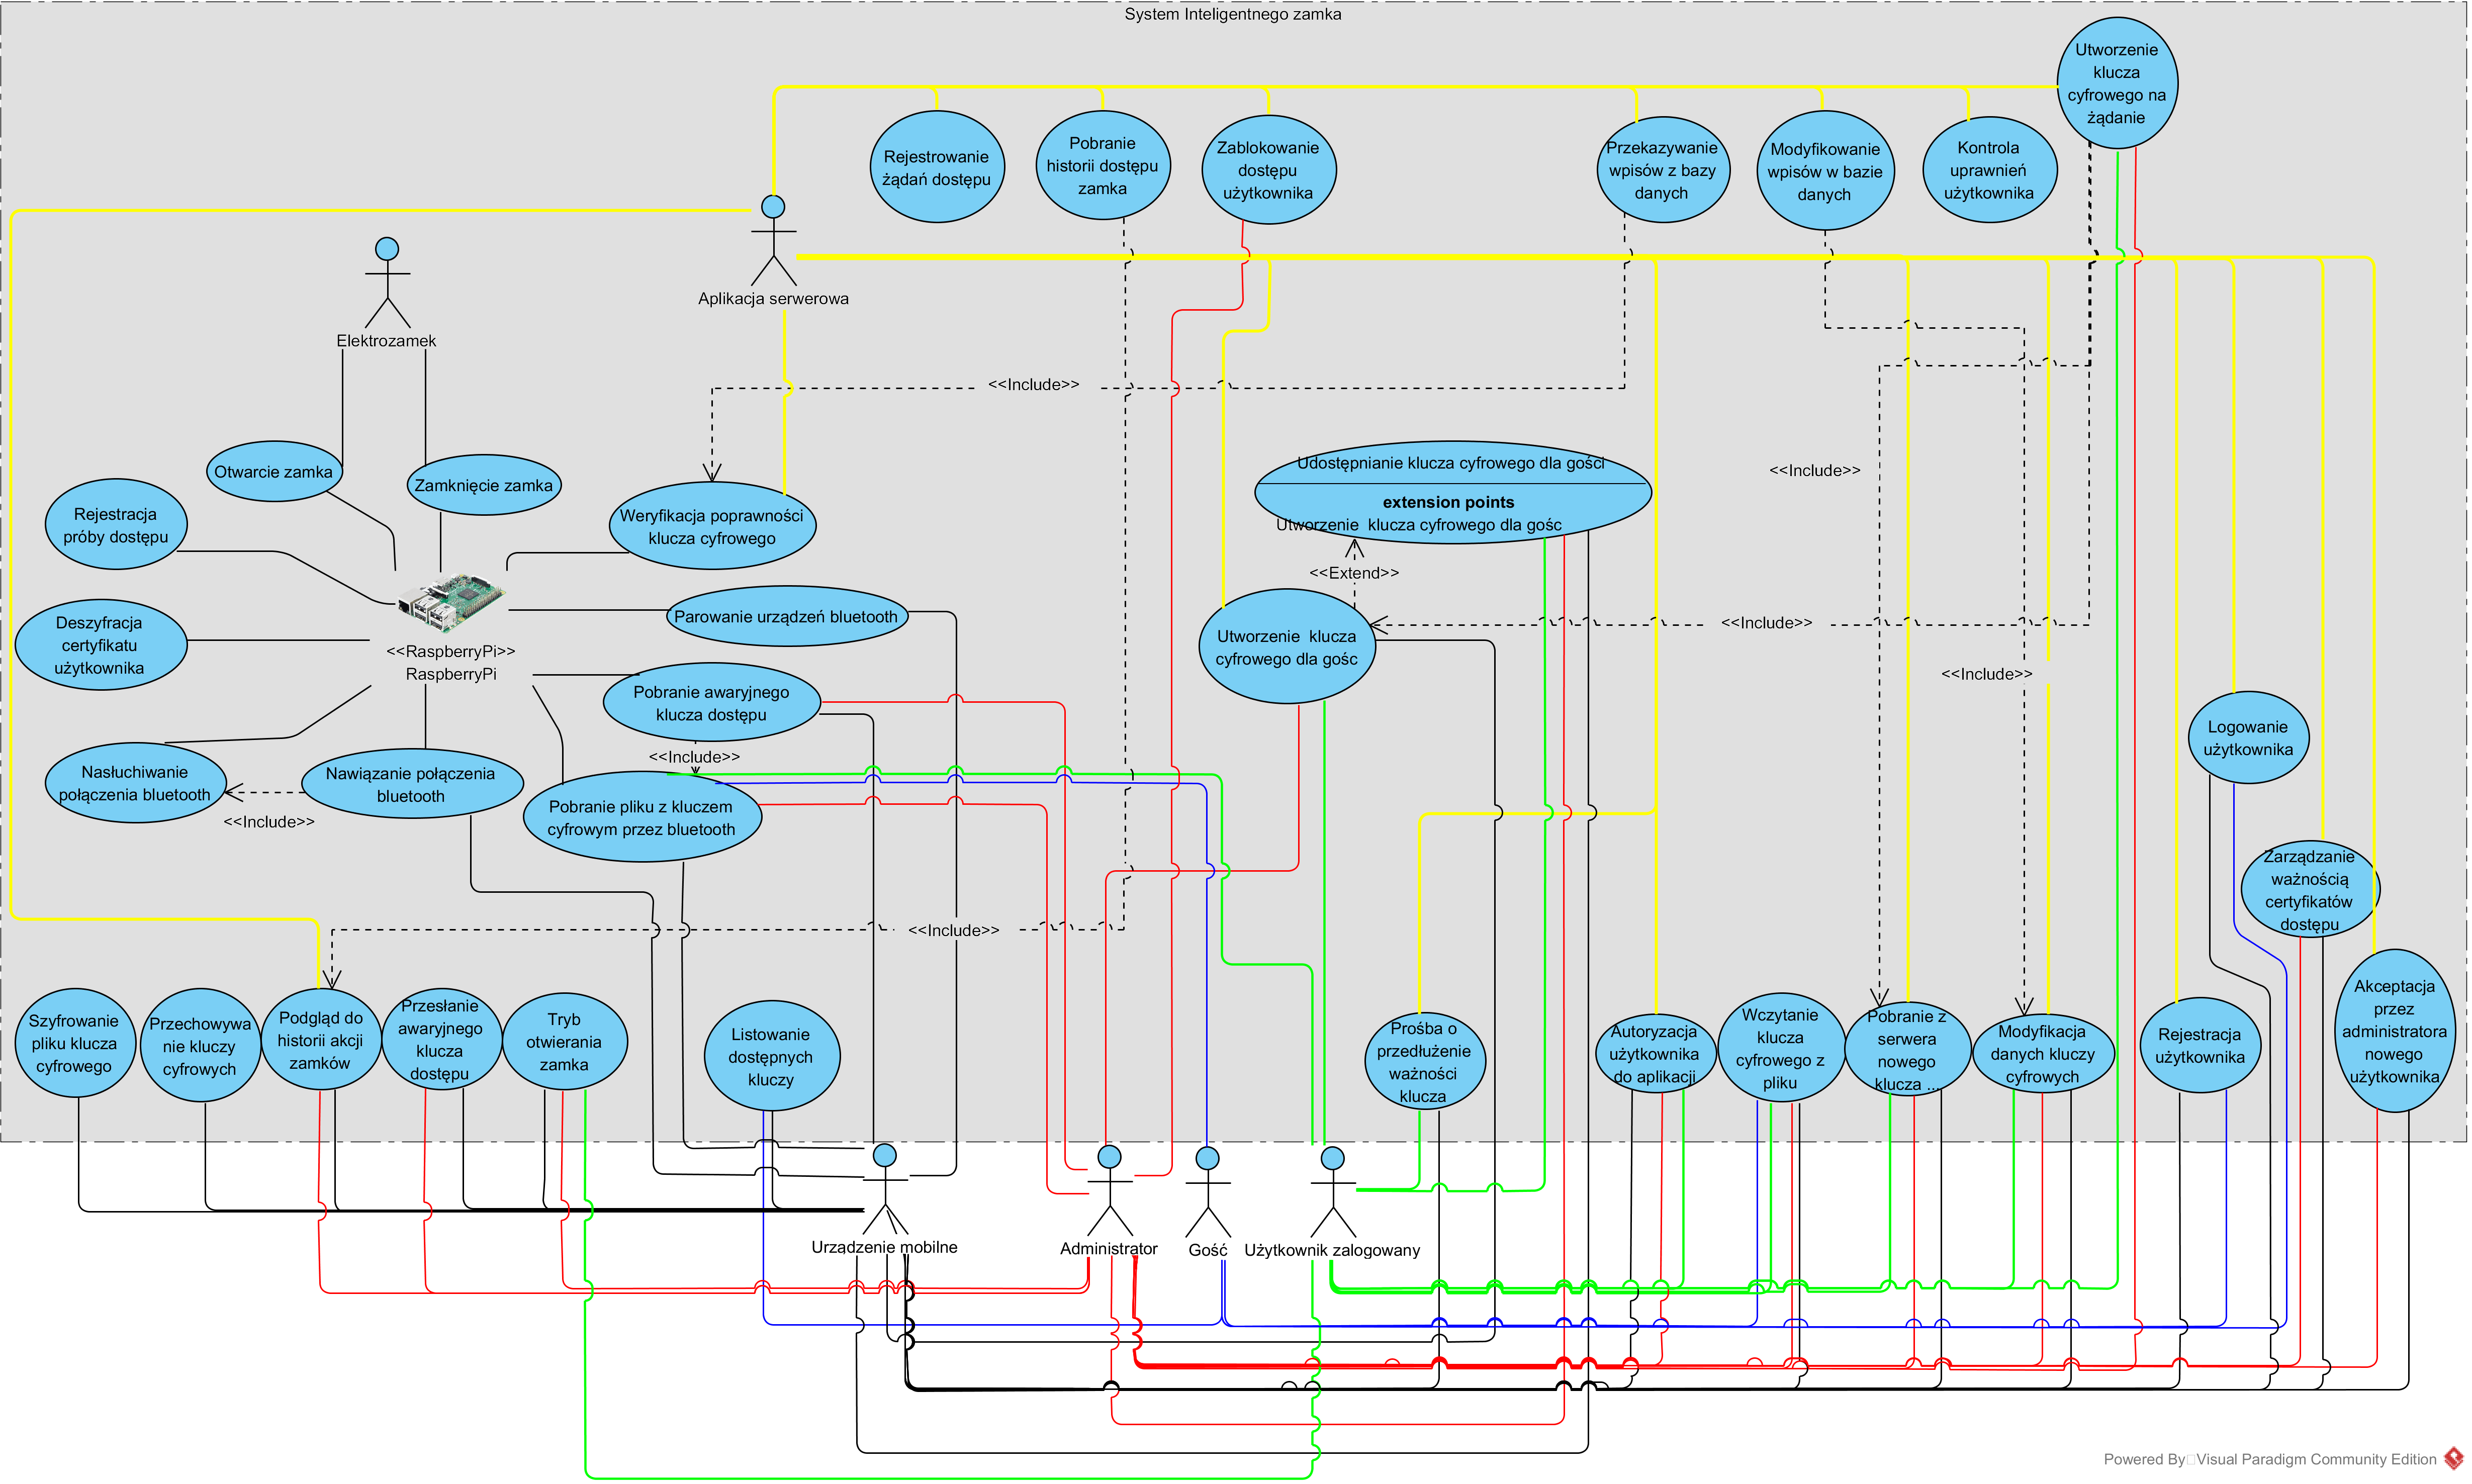
\includegraphics[width=22cm]{Obrazy/Diagram_przypadkow_uzycia.png}
			\caption{Diagram przypadków użycia}
			\label{diagram:diagram przypadków_użycia}
		\end{figure}
	\end{landscape}
\newpage
	\subsubsection{Projekt bazy danych [Maciej Marciniak]} 
	Baza danych będzie składać się z pięciu tabel:
	\begin{itemize*}
		\item {USERS} --- przechowuje dane użytkowników oraz dane niezbędne przy weryfikacji logowania,
		\item {LOCKS} --- zawiera informacje na temat dostępnych w systemie zamków,
		\item {ACCESS\_TO\_LOCKS} --- archiwizuje próby użycia certyfikatów,
		\item {LOCKS\_KEYS} --- zawiera wszystkie klucze dostępowe użytkowników,
		\item {WAIT\_LOCKS\_KEYS} --- przetrzymuje klucze dostępowe oczekujące na zatwierdzenie przez administratora.
	\end{itemize*}
	
	Wiersz tabeli USERS zawierać musi:
	\begin{itemize*}
		\item {ID\_USER} --- unikalny identyfikator (klucz główny) użytkownika składający się z 10 cyfr,
		\item {LOGIN} --- unikalna nazwa użytkownika niezbędna podczas logowania, zawierająca nie więcej niż 255 znaków,
		\item {PASSWORD} --- hasło zapisane w postaci skrótu, potrzebne do autoryzacji dostępu użytkownikowi,
		\item {NAME} - imię użytkownika,
		\item {SURNAME} --- nazwisko użytkownika,
		\item {TOKEN} --- generowany ciąg pseudolosowy klucz sesji logowania,
		\item  {ISACTIVATED} --- pole boolowskie oznaczające, czy dane konto jest zaakceptowane,
		\item {IS\_ADMIN} --- pole boolowskie wskazujące czy dany użytkownik jest administratorem czy nie, (aktywowane) przez administratora.
		\item {PUBLIC\_KEY} --- klucz publiczny użytkownika potrzebny do podpisu cyfrowego,
		\item Serial\_number --- unikalny numer seryjny certyfikatu szyfrującego,
		\item Validity\_period --- data do której ważny jest certyfikat szyfrujący,
		\item Version --- numer wersji certyfikatu szyfrującego,
		\item Signature\_Algorithm\_Identifier --- identyfikator algorytmu szyfrującego,
		\item Hash\_Algorithm --- identyfikator algorytmu funkcji skrótu.
	\end{itemize*}
	
	Zamek opisywany jest poprzez kolumny:
	\begin{itemize*}
		\item {ID\_LOCK} --- unikalny identyfikator (klucz główny) zamka składający się z 10 cyfr,
		\item {NAME} --- unikalna nazwa zamka,
		\item {MAC\_ADDRESS} --- adres fizyczny urządzenia sterującego zamkiem,
		\item {LOCALIZATION} --- nieobowiązkowe pole opisujące fizyczne położenie zamka,
		\item {People\_inside} --- wartość licznika osób znajdujących się wewnątrz pomieszczenia.
	\end{itemize*}
	\newpage
	
	Klucz dostępowy składa się z:
	\begin{itemize*}
		\item {ID\_KEY} --- unikalny identyfikator (klucz główny) klucza dostępowego składający się z 10 cyfr,
		\item {ID\_LOCK} --- klucz obcy do tabeli przechowującej dostępne zamki,
		\item {ID\_USER} --- klucz obcy do tabeli przechowującej dane użytkownika, jest to pole służące do określenia kto utworzył klucz dostępu,
		\item {LOCK\_KEY} --- unikalna wartość certyfikatu dostępu,
		\item {FROM\_DATE} --- data od której obowiązuje klucz,
		\item {TO\_DATE} --- data do której obowiązuje klucz,
		\item {ISACTUAL} --- data wygaśnięcia klucza, jeśli równa TO, oznacza to że klucz utracił ważność z powodu czasu, jeśli różna oznacza, to że zablokowano z innego powodu ważność,
		\item {MONDAY} --- słowne określenie, w których godzinach zostanie przyznany dostęp w poniedziałki,
		\item {TUESDAY} --- słowne określenie, w których godzinach zostanie przyznany dostęp we wtorki,
		\item {WEDNESDAY} --- słowne określenie, w których godzinach zostanie przyznany dostęp w środy,
		\item {THURSDAY} --- słowne określenie, w których godzinach zostanie przyznany dostęp w czwartki,
		\item {FRIDAY} --- słowne określenie, w których godzinach zostanie przyznany dostęp w piątki,
		\item {SATURDAY} --- słowne określenie, w których godzinach zostanie przyznany dostęp w soboty,
		\item {SUNDAY} --- słowne określenie, w których godzinach zostanie przyznany dostęp w niedziele,
		\item {IS\_PERNAMENT} --- zmienna boolowska oznaczająca czy dostęp jest zawsze,
		\item {NAME} - imię osoby, której dotyczy certyfikat,
		\item {SURNAME} --- nazwisko osoby, której dotyczy certyfikat.
	\end{itemize*}
	
	W tabeli archiwizującej akcje na zamku znajdują się takie dane jak:
	\begin{itemize*}
		\item {ID} --- unikalny identyfikator (klucz główny) akcji wykonanej na certyfikacie składający się z 10 cyfr,
		\item {ID\_KEY} --- klucz obcy do tabeli przechowującej klucze dostępowe, dzięki tej informacji możemy uzyskać dane o zamku, który został otwierany jak również do kogo należał klucz,
		\item {DATE} --- dokładna data z godziną użycia klucza dostępowego,
		\item {ACCESS} --- binarna flaga informująca czy dostęp został przyznany czy odmówiony.
	\end{itemize*}
\newpage
	Tabela WAIT\_LOCKS\_KEYS składa się z:
	\begin{itemize*}
		\item {ID\_KEY} --- unikalny identyfikator (klucz główny) oczekującego certyfikatu,
		\item{ID\_LOCK} --- klucz obcy do tabeli LOCKS, oznacza zamek do którego jest zgłaszana prośba dostępu,
		\item {ID\_USER} --- klucz obcy do tabeli USERS, oznacza użytkownika który zgłasza prośbę o dostęp do zamka.
	\end{itemize*}
	
	Diagramy bazy danych odpowiednio encji i relacji przedstawione zostały na Rys \ref{diagram:diagram encji} i Rys. \ref{diagram:diagram relacji}.  
	
	\begin{figure}[!h]
		\centering
		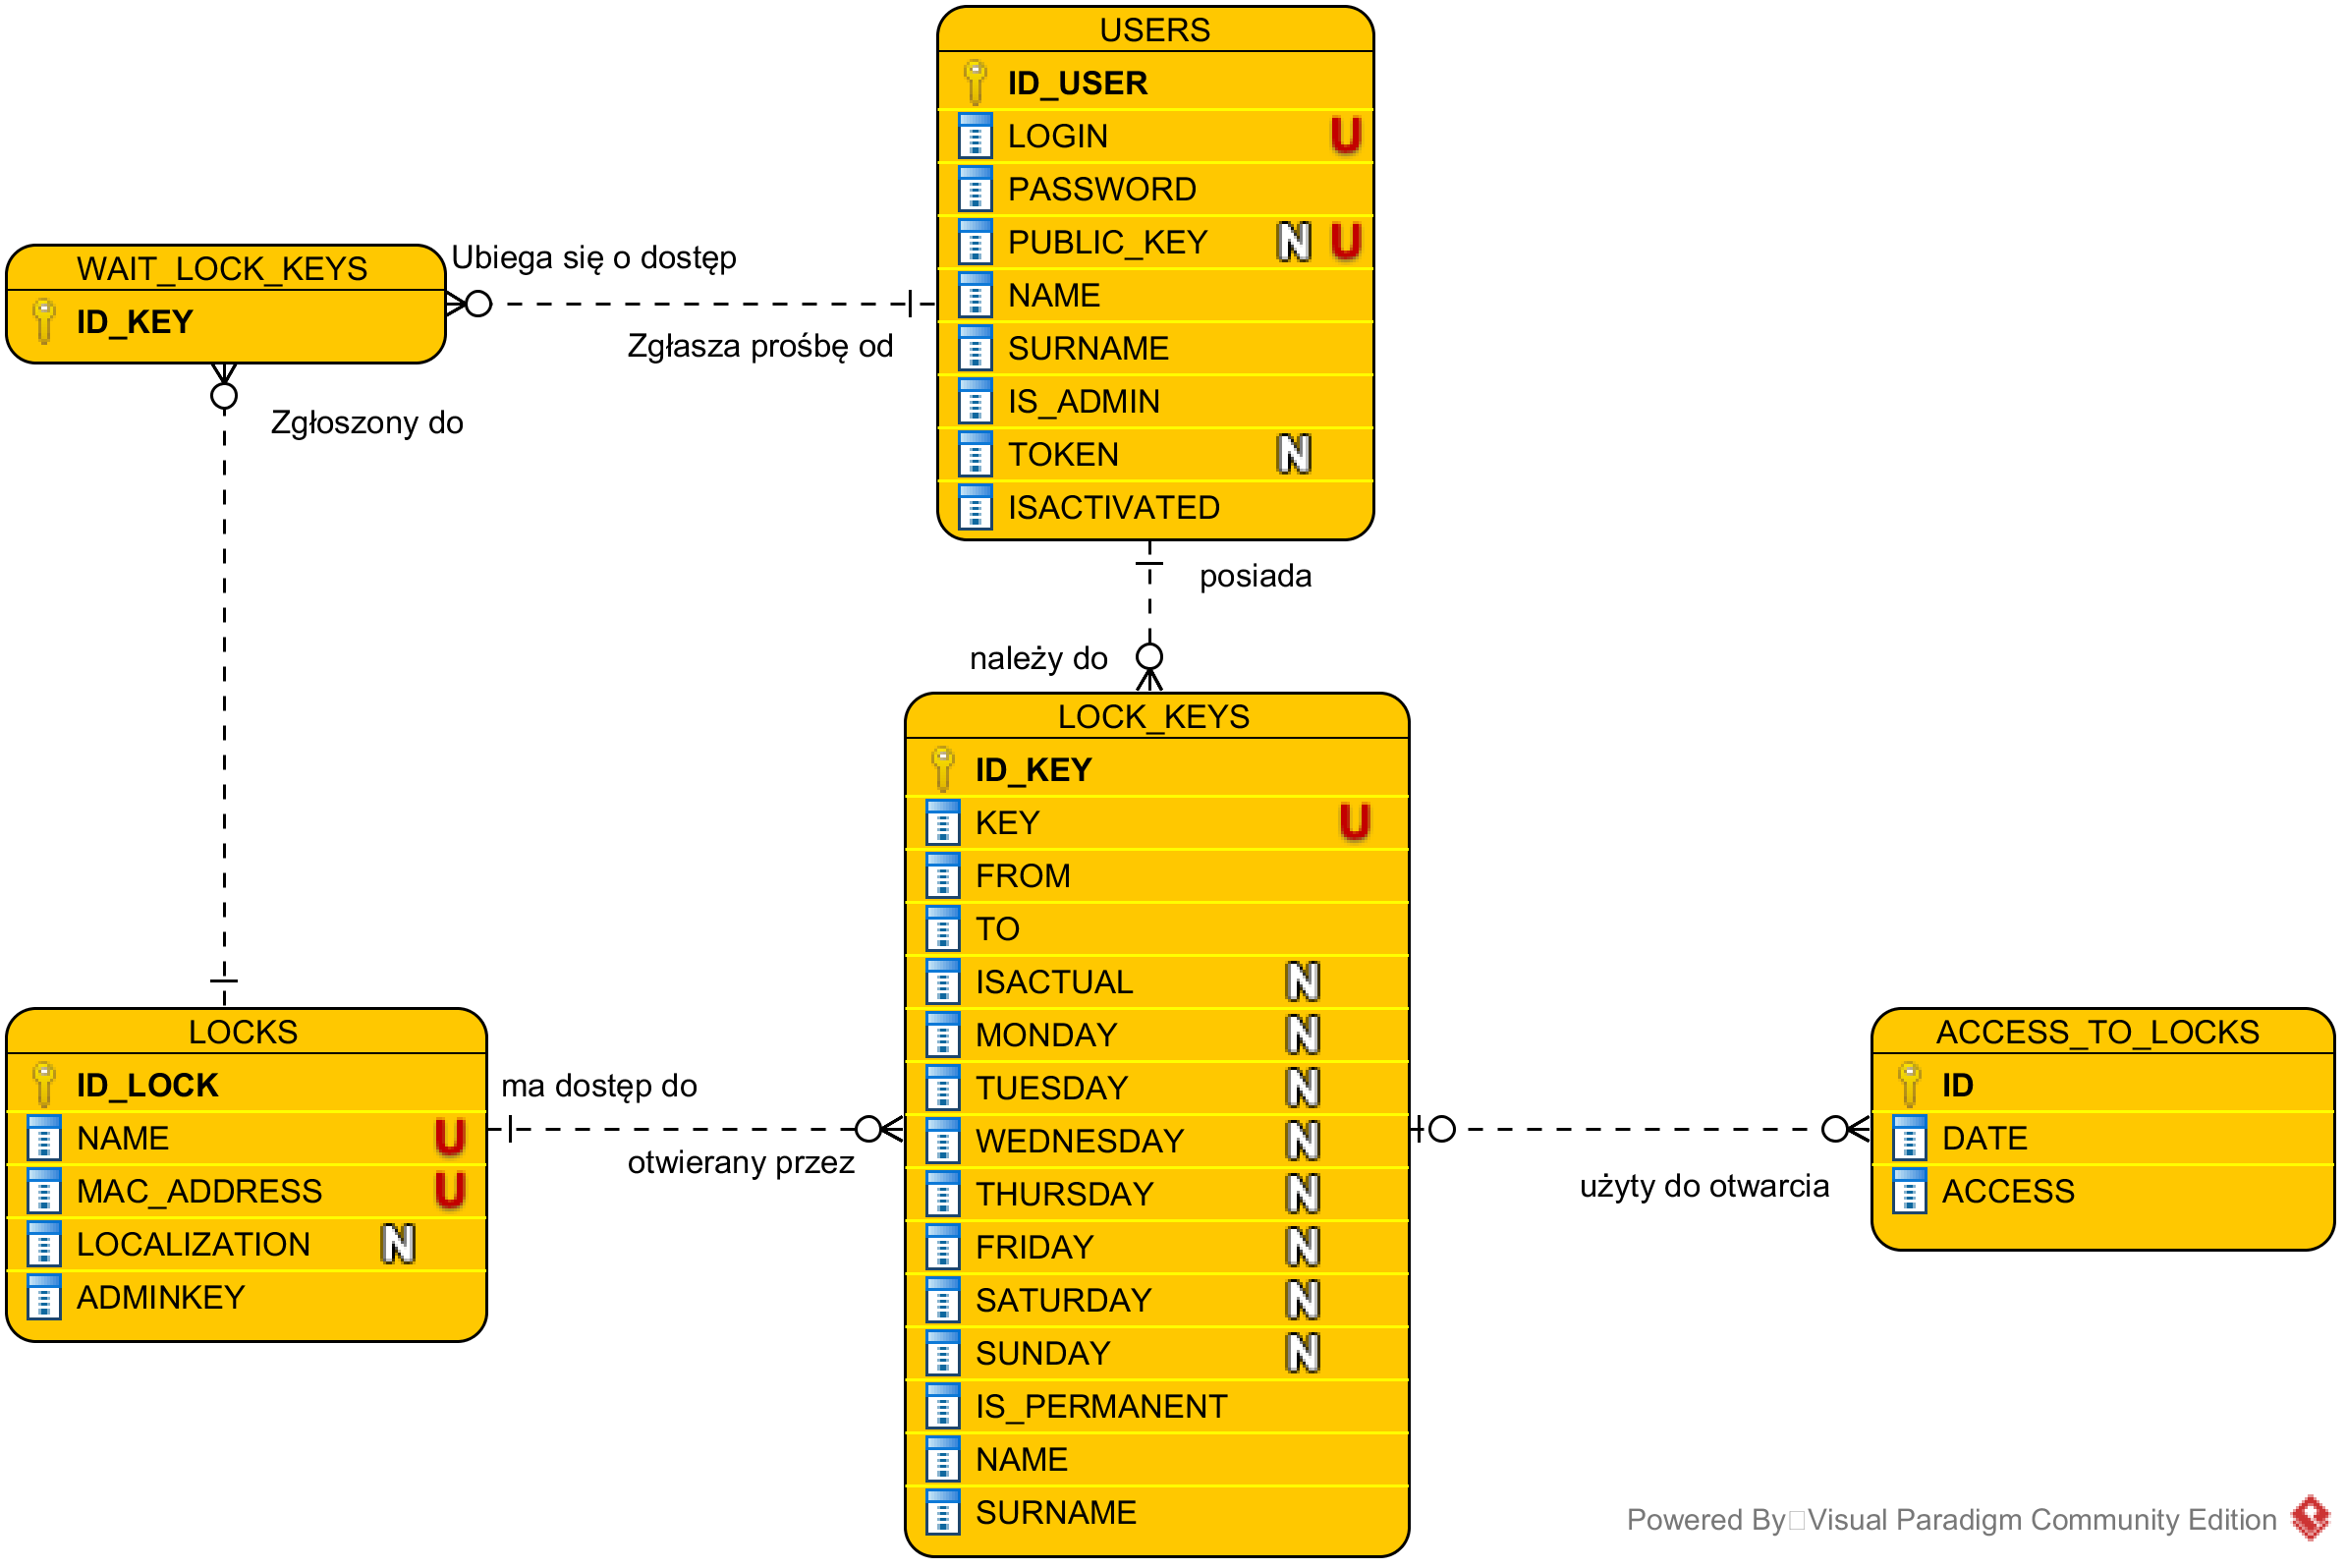
\includegraphics[width=13cm]{Obrazy/Diagram_encji.png}
		\caption{Diagram encji bazy danych}
		\label{diagram:diagram encji}
	\end{figure}
	\newpage
	\begin{figure}[!h]
		\centering
		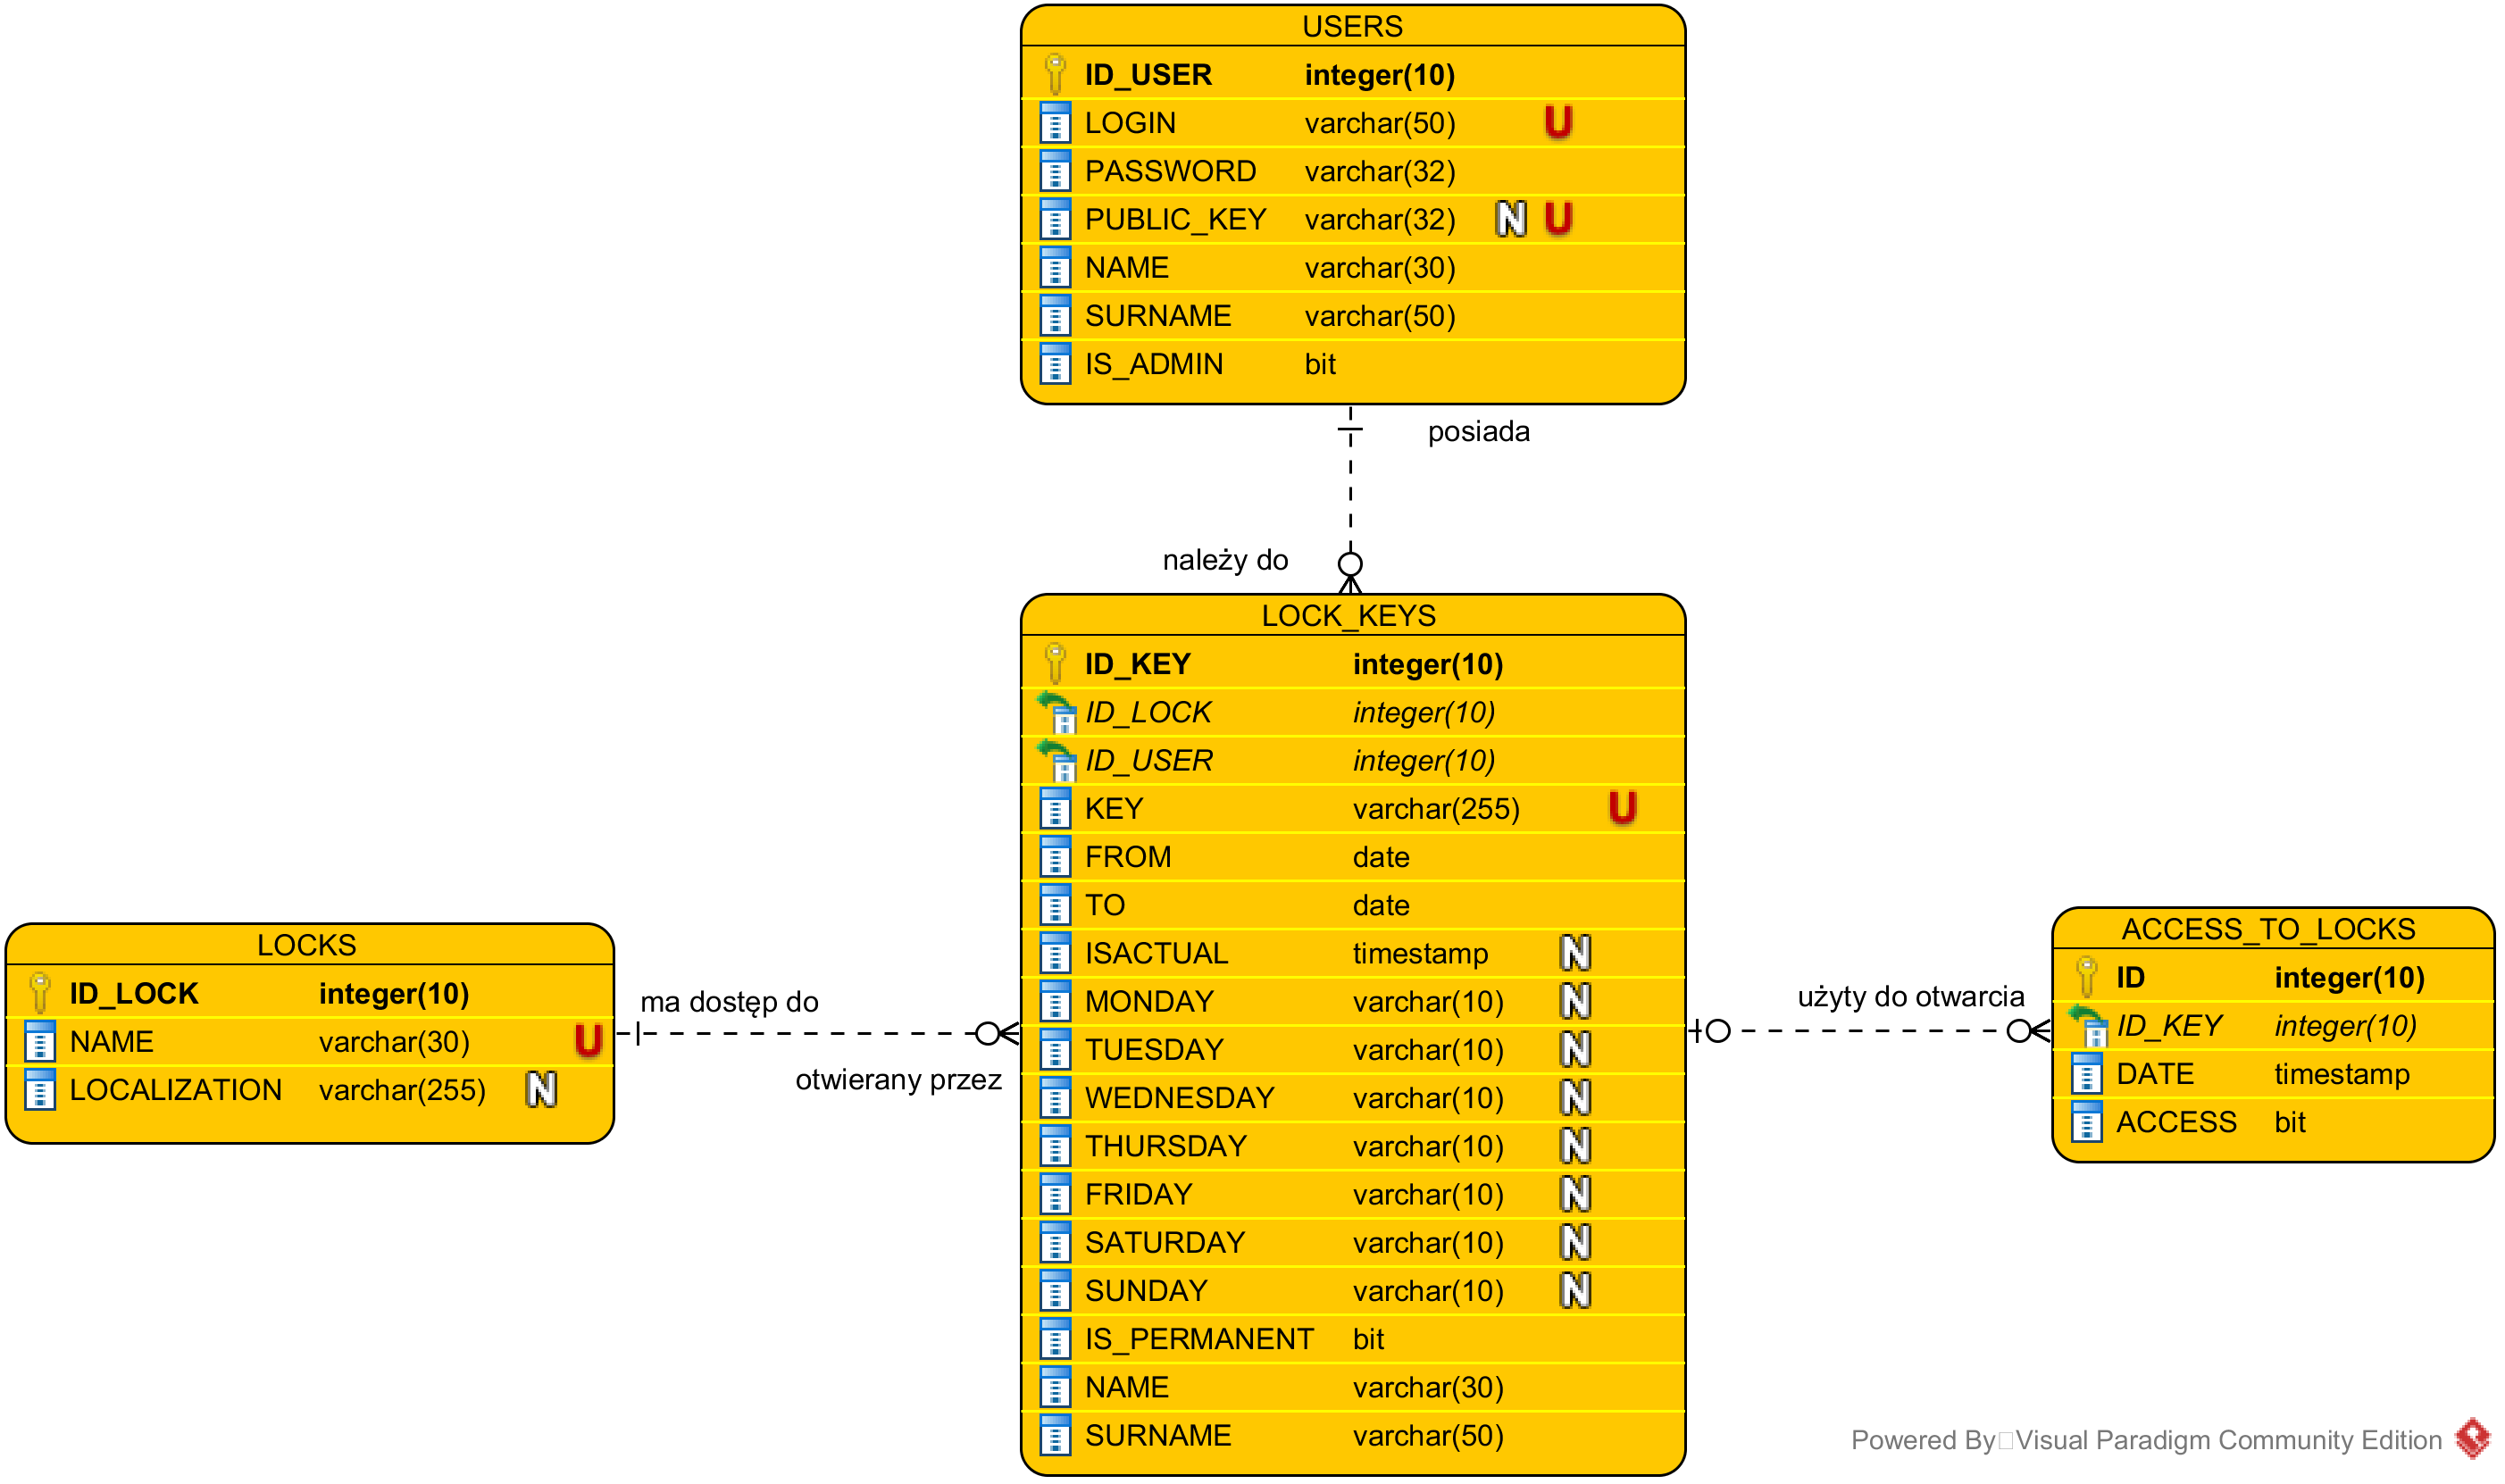
\includegraphics[width=13cm]{Obrazy/Diagram_relacji.png}
		\caption{Diagram relacji bazy danych}
		\label{diagram:diagram relacji}
	\end{figure}
\newpage

	\subsubsection{Diagramy klas}
		\paragraph*{Aplikacja mobilna [Damian Filipowicz]}
		Aplikacja mobilna składa się z szeregu klas napisanych w 2 językach: Kotlin oraz Java. Ponadto klasy te zostały podzielone na 5 kategorii (Rys. \ref{Schemat ogólny diagramu klas dla Aplikacji mobilnej}) takich jak:
		\begin{itemize*}
			\item API 
			(Rys. \ref{Diagram klas dla paczki api}) 
			---  które przechowuje klasy odpowiedzialne za funkcje wykorzystywane w wielu miejscach systemu. W paczce znajdują się klasy odpowiedzialne między innymi za odczyt oraz zapis do pliku, komunikacje HTTPS, czy wykorzystywanie SharedPreferences w aplikacji ,
			\item Navigation 
			(Rys. \ref{Diagram klas dla paczki navigations}) 
			--- są to klasy odpowiedzialne za generowanie nawigacji w aplikacji mobilnej. Paczka znajdują się 4 klasy,
			\item Adapters
			(Rys. \ref{Diagram klas dla paczki adapters}) 
			 --- w którym są przechowywane klasy adapter wykorzystywane w systemie do wyświetlania danych,
		\end{itemize*}
	
	\begin{figure}[ht!]
		\centering
		\vspace{-0.6cm}
		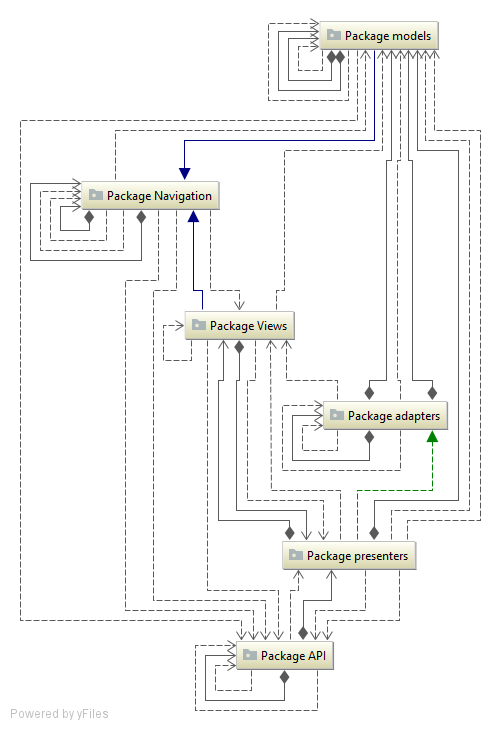
\includegraphics[width=7.8cm]{Obrazy/AM_DK_ALL}
		\caption{Schemat ogólny diagramu klas dla Aplikacji Mobilnej}
		\label{Schemat ogólny diagramu klas dla Aplikacji mobilnej}
	\end{figure}
	\newpage
\begin{figure}[ht!]
	\centering
	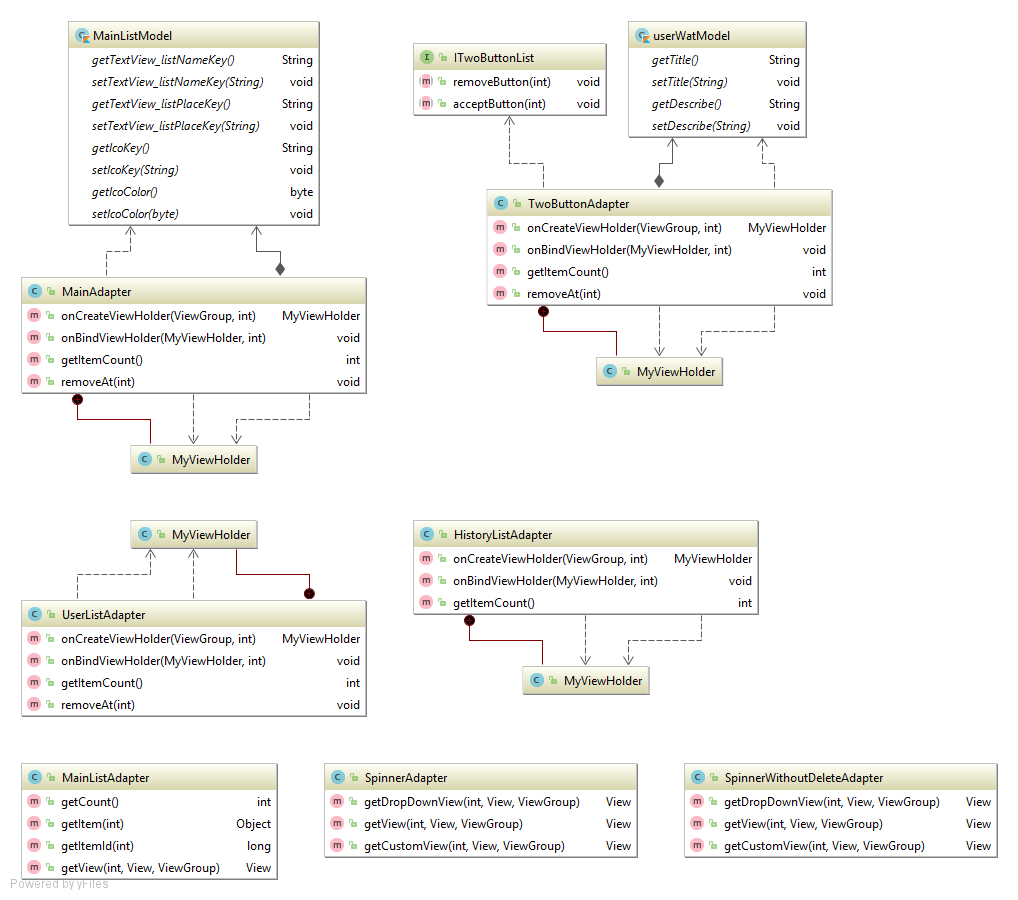
\includegraphics[width=12.5cm]{Obrazy/AM_DK_adapter}
	\caption{Diagram klas dla paczki adapters}
	\label{Diagram klas dla paczki adapters}
\end{figure}
\newpage
\begin{figure}[ht!]
	\centering
	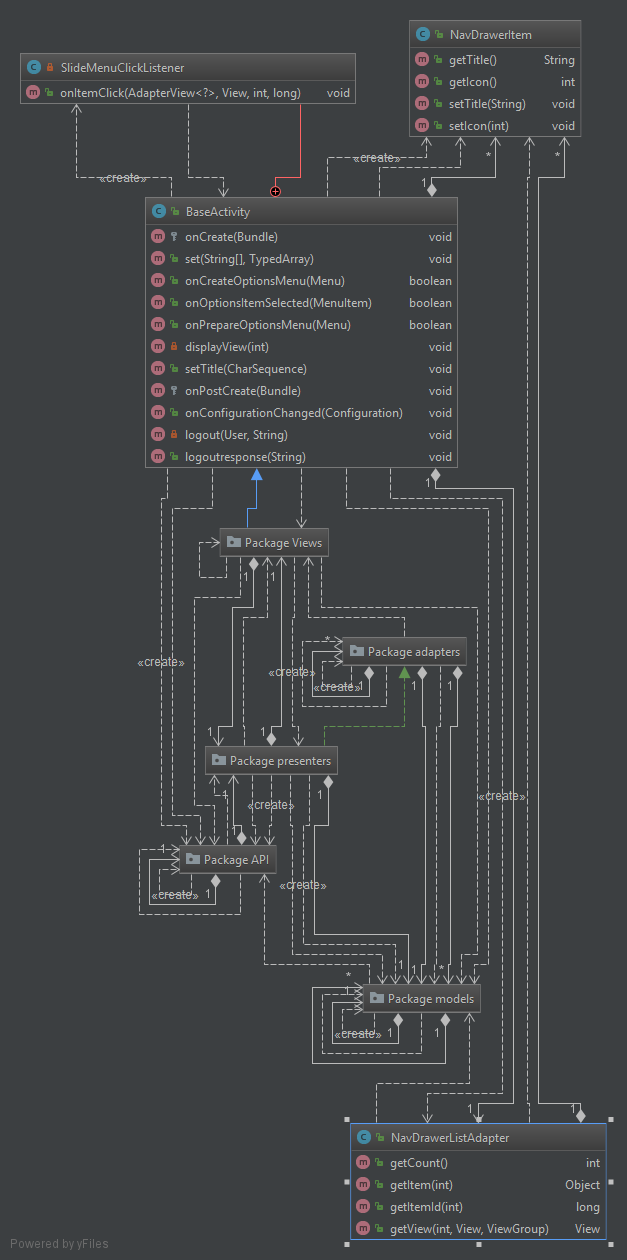
\includegraphics[width=12.5cm]{Obrazy/AM_DK_navigation}
	\caption{Diagram klas dla paczki navigations}
	\label{Diagram klas dla paczki navigations}
\end{figure}
\newpage
\begin{figure}[ht!]
	\centering
	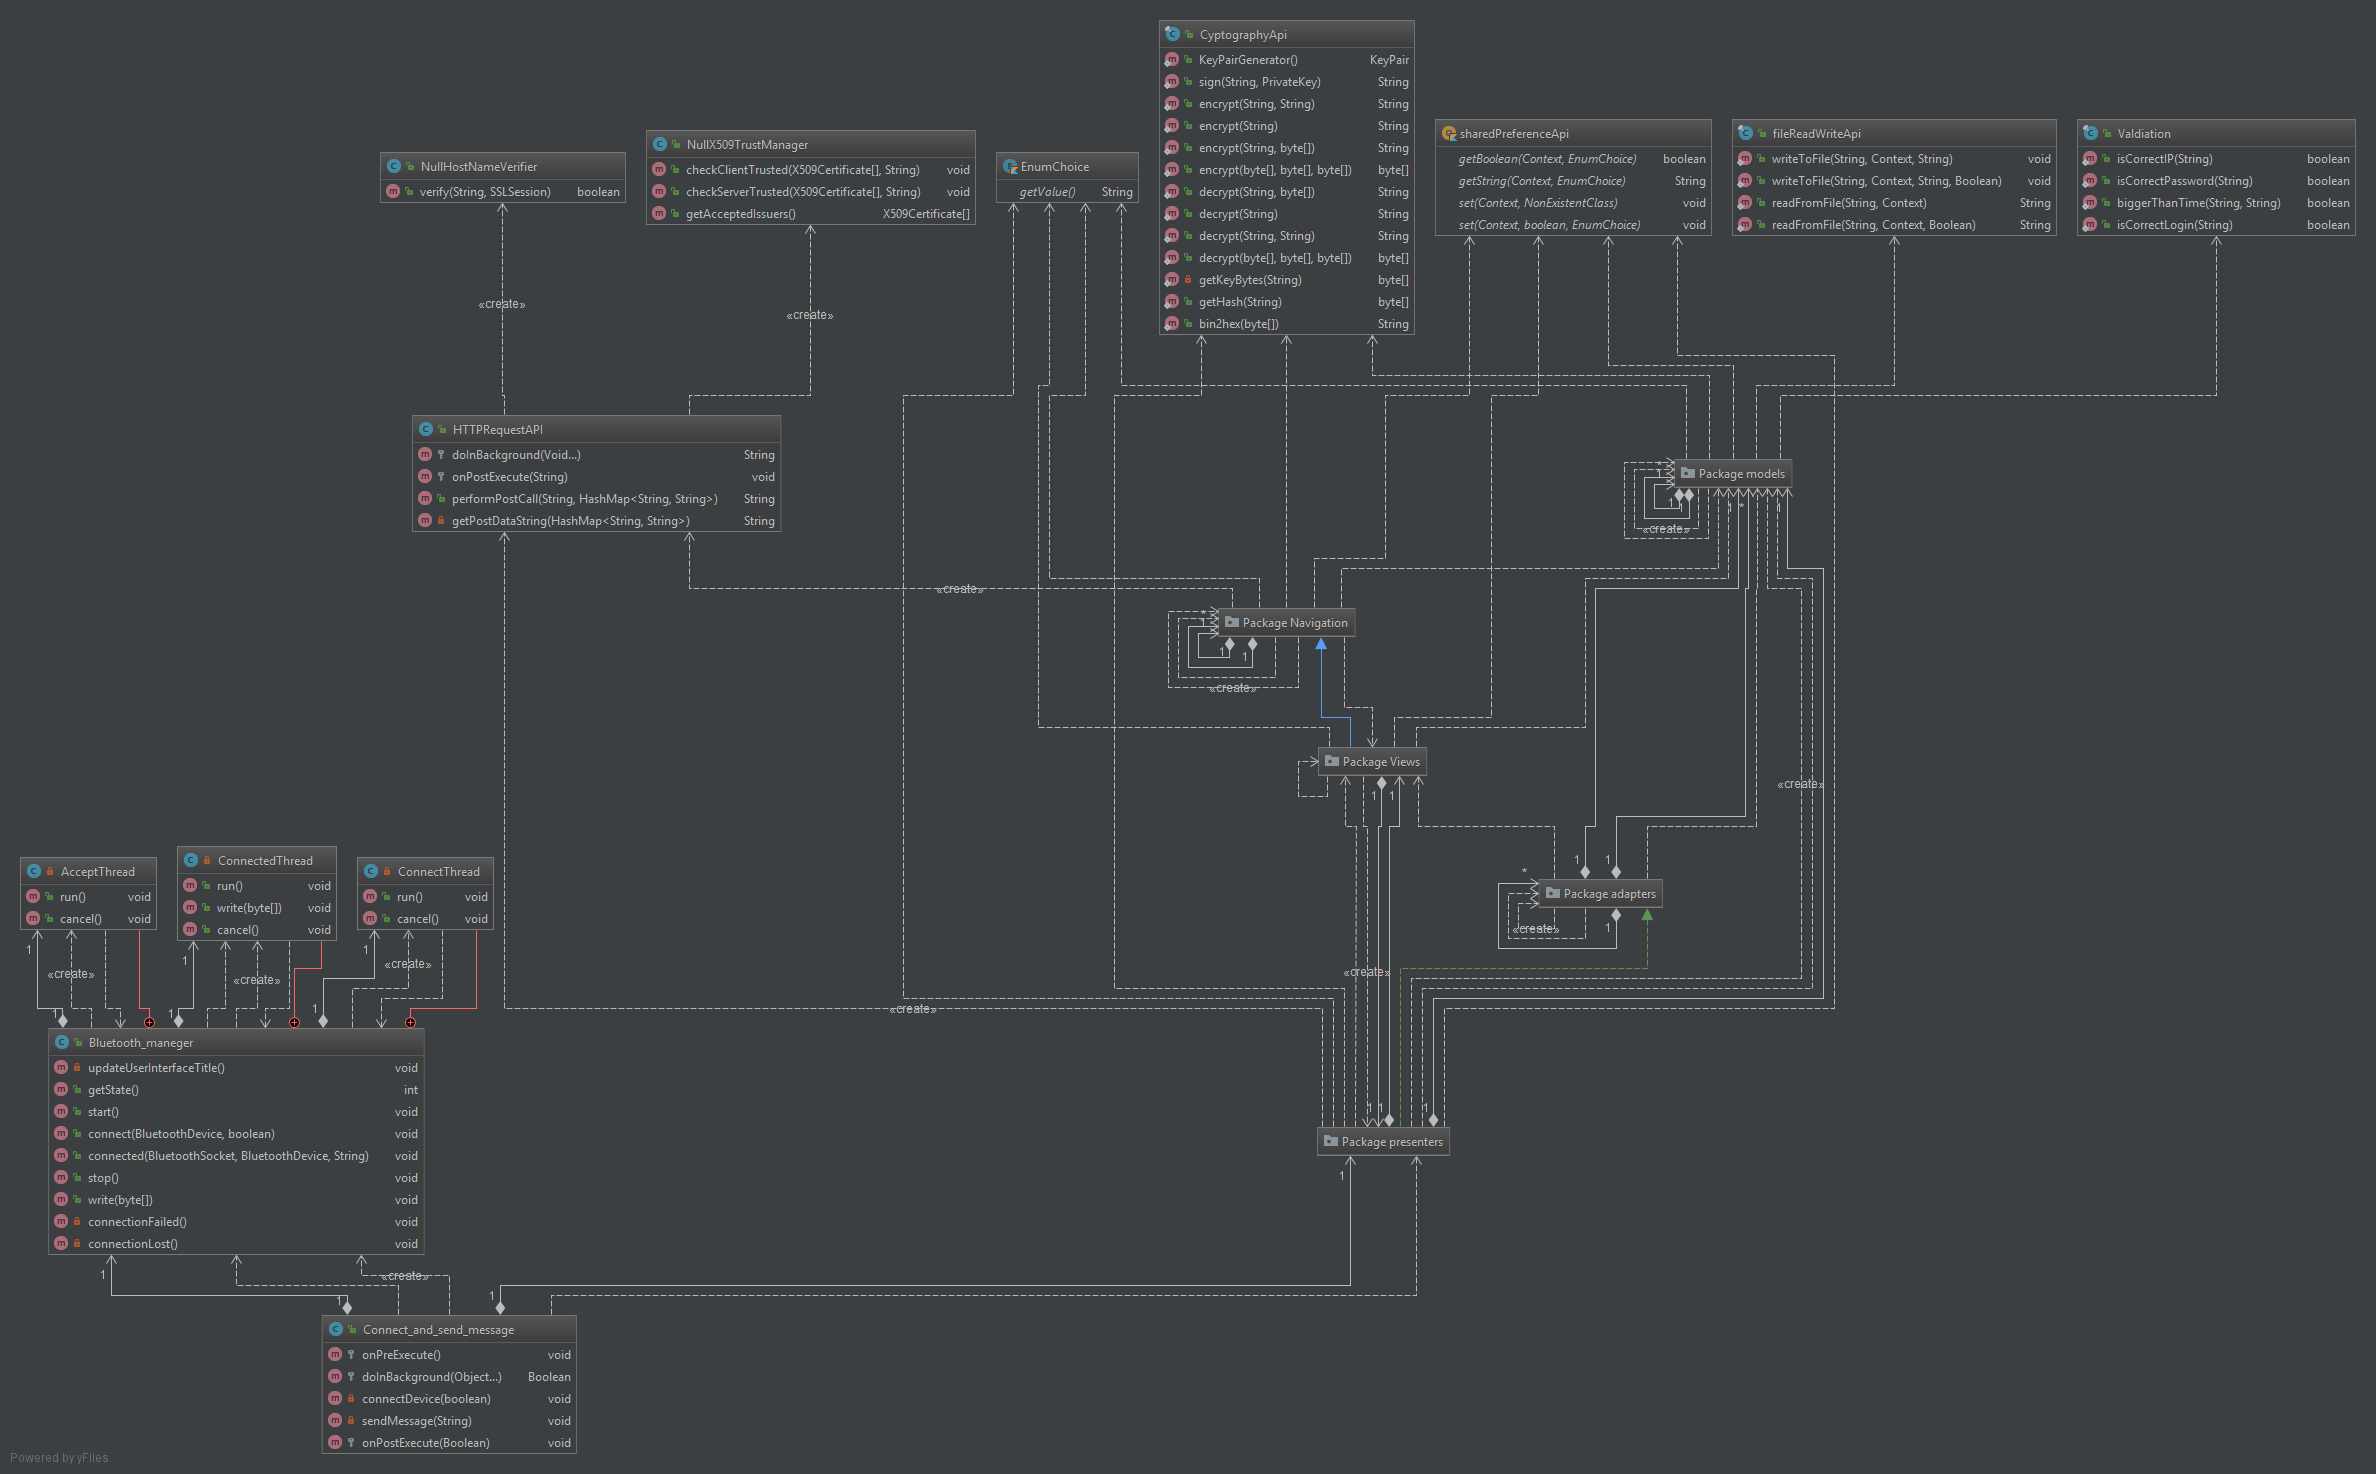
\includegraphics[width=12.5cm]{Obrazy/AM_DK_api}
	\caption{Diagram klas dla paczki api}
	\label{Diagram klas dla paczki api}
\end{figure}
\newpage
Oprócz tych wymienionych wyżej są dodatkowo 3 kategorie implementujące wzorzec architektoniczny Model-View-Presenter i są to odpowiednio:
\begin{itemize*}
	\item Model (Rys. \ref{Diagram klas dla paczki models}) 
				 --- przechowujący klasy modele odpowiedzialne za przechowywanie danych. Każda z klas która jest powiązana z odpowiednim widokiem   w nazwie na początku ma nazwę widoku a na końcu ma słowo Model,   
				\item View 
				(Rys. \ref{Diagram klas dla paczki views}) 
				--- przechorowujący klasy widoków odpowiedzialne za generowanie widoków w aplikacji. Każda z klas która jest powiązana z odpowiednim widokiem   w nazwie na początku ma nazwę widoku a na końcu ma słowo Activity, 
				\item Presenter
				(rysunek \ref{Diagram klas dla paczki presenters}) 
				 --- przechowujący klasy presenter odpowiedzialne za interakcje pomiędzy modelami oraz widokami. Każda z klas, która jest powiązana z odpowiednim widokiem w nazwie na początku ma nazwę widoku, a na końcu ma słowo Presenter.
\end{itemize*}
		\newpage
	\begin{figure}[ht!]
		\centering
		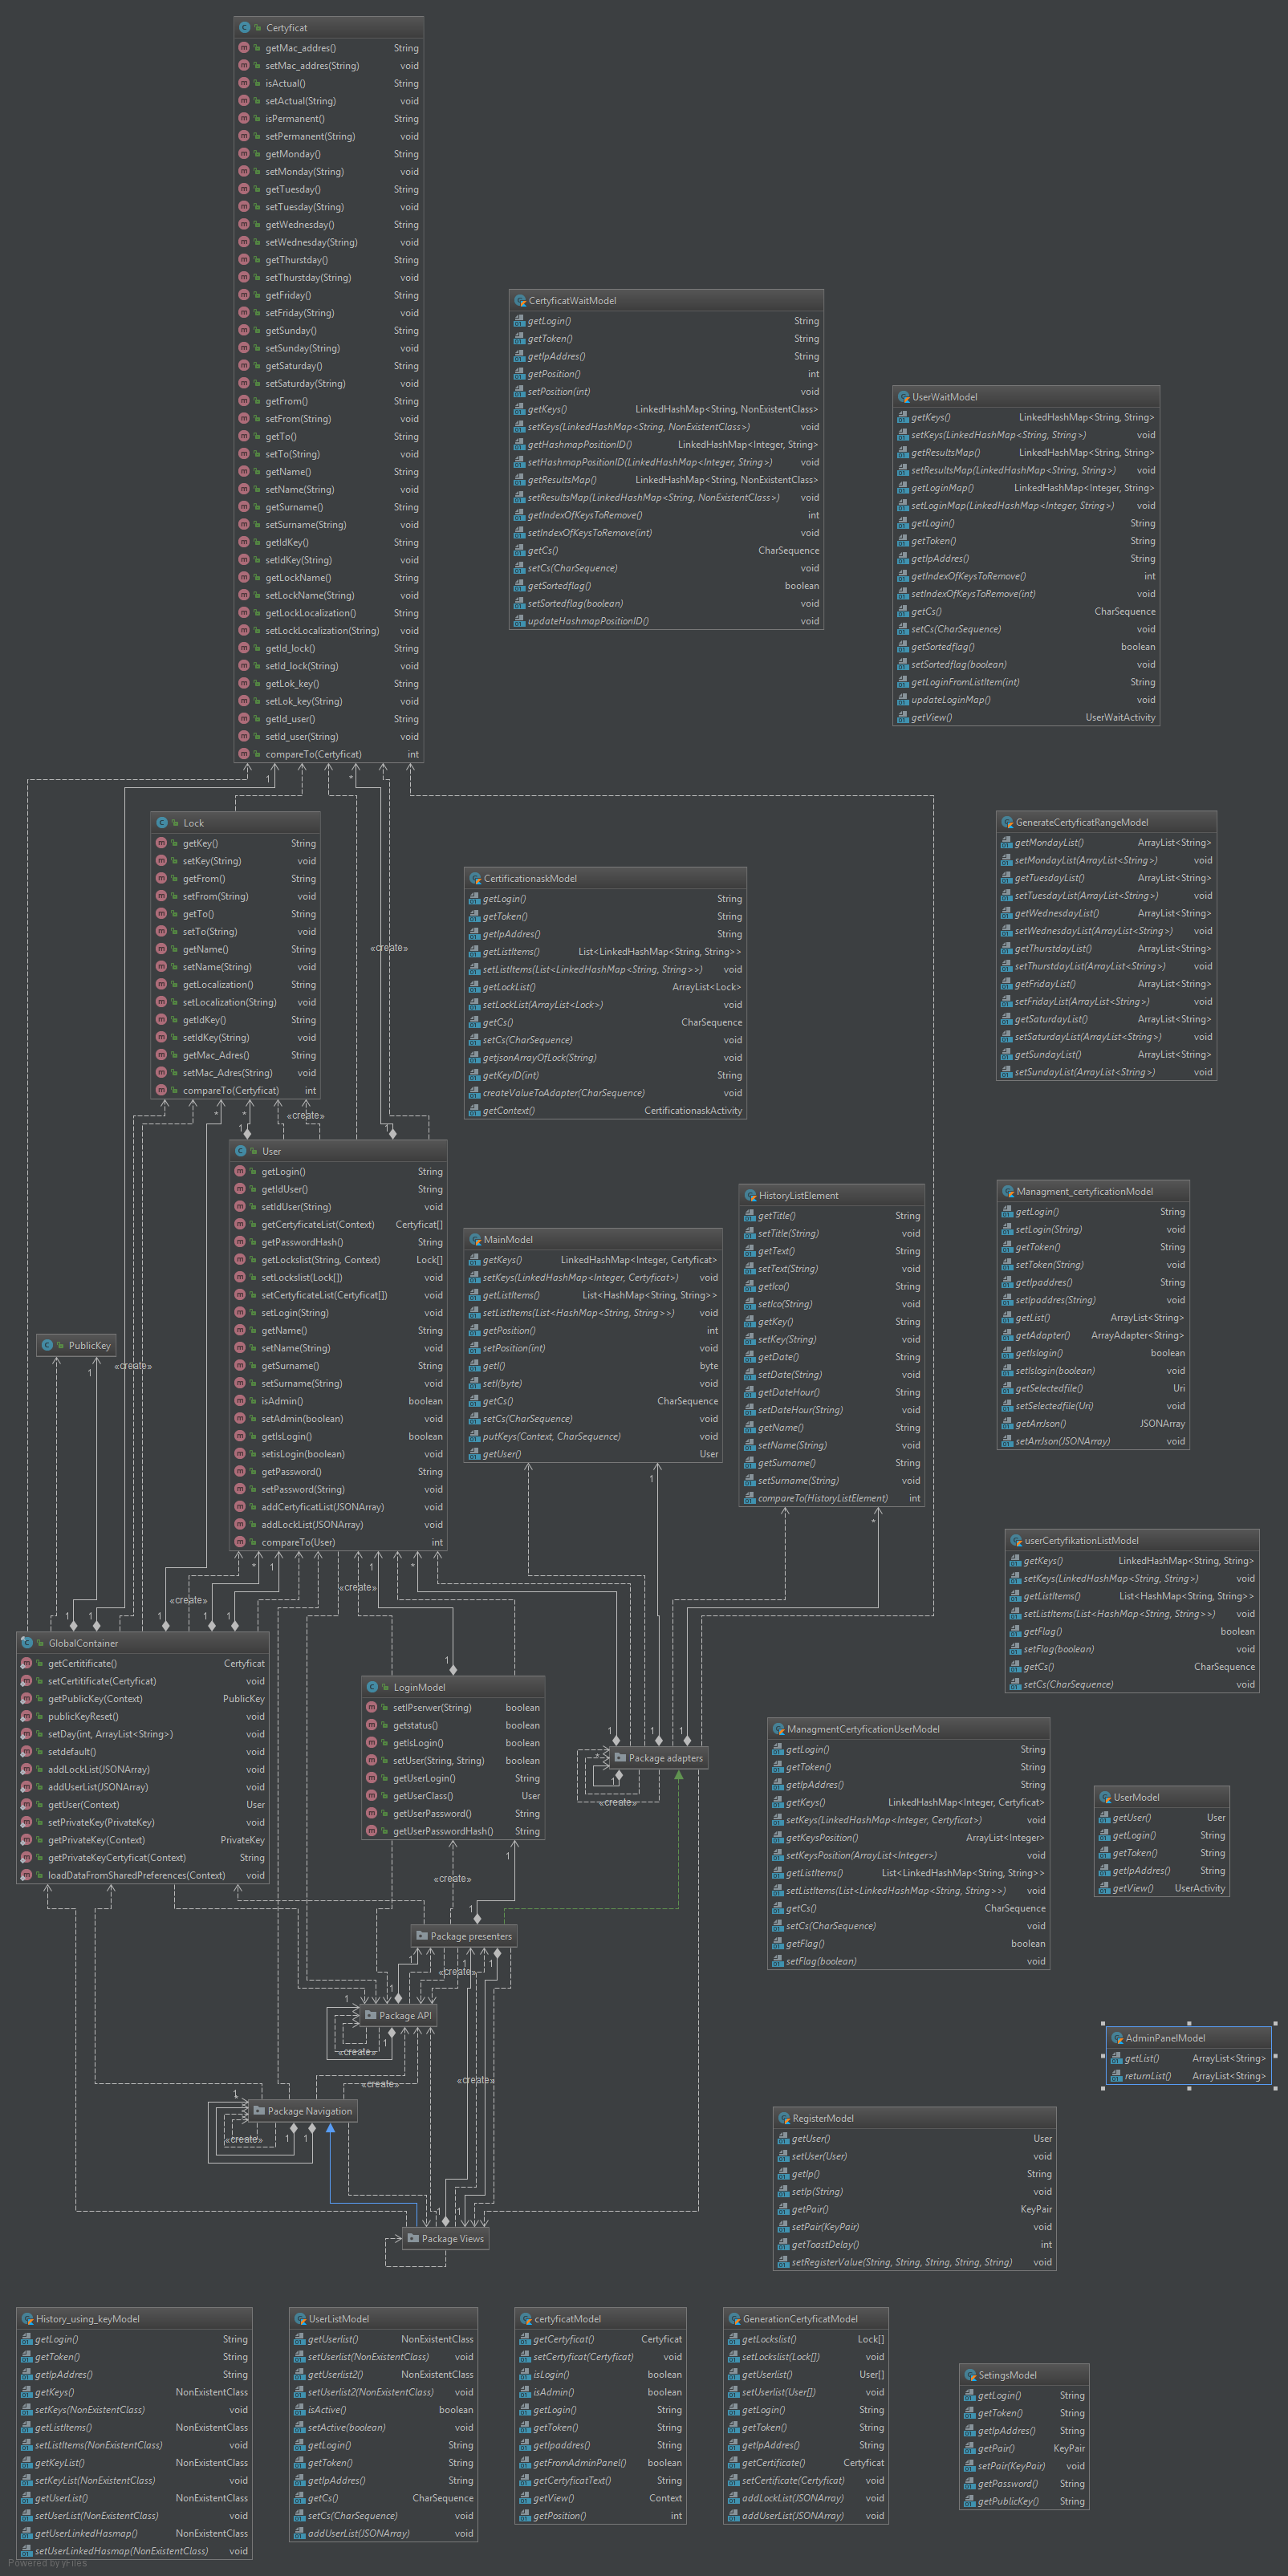
\includegraphics[width=12cm]{Obrazy/AM_DK_model}
		\caption{Diagram klas dla paczki models}
		\label{Diagram klas dla paczki models}
	\end{figure}

	\newpage
\begin{figure}[ht!]
	\centering
	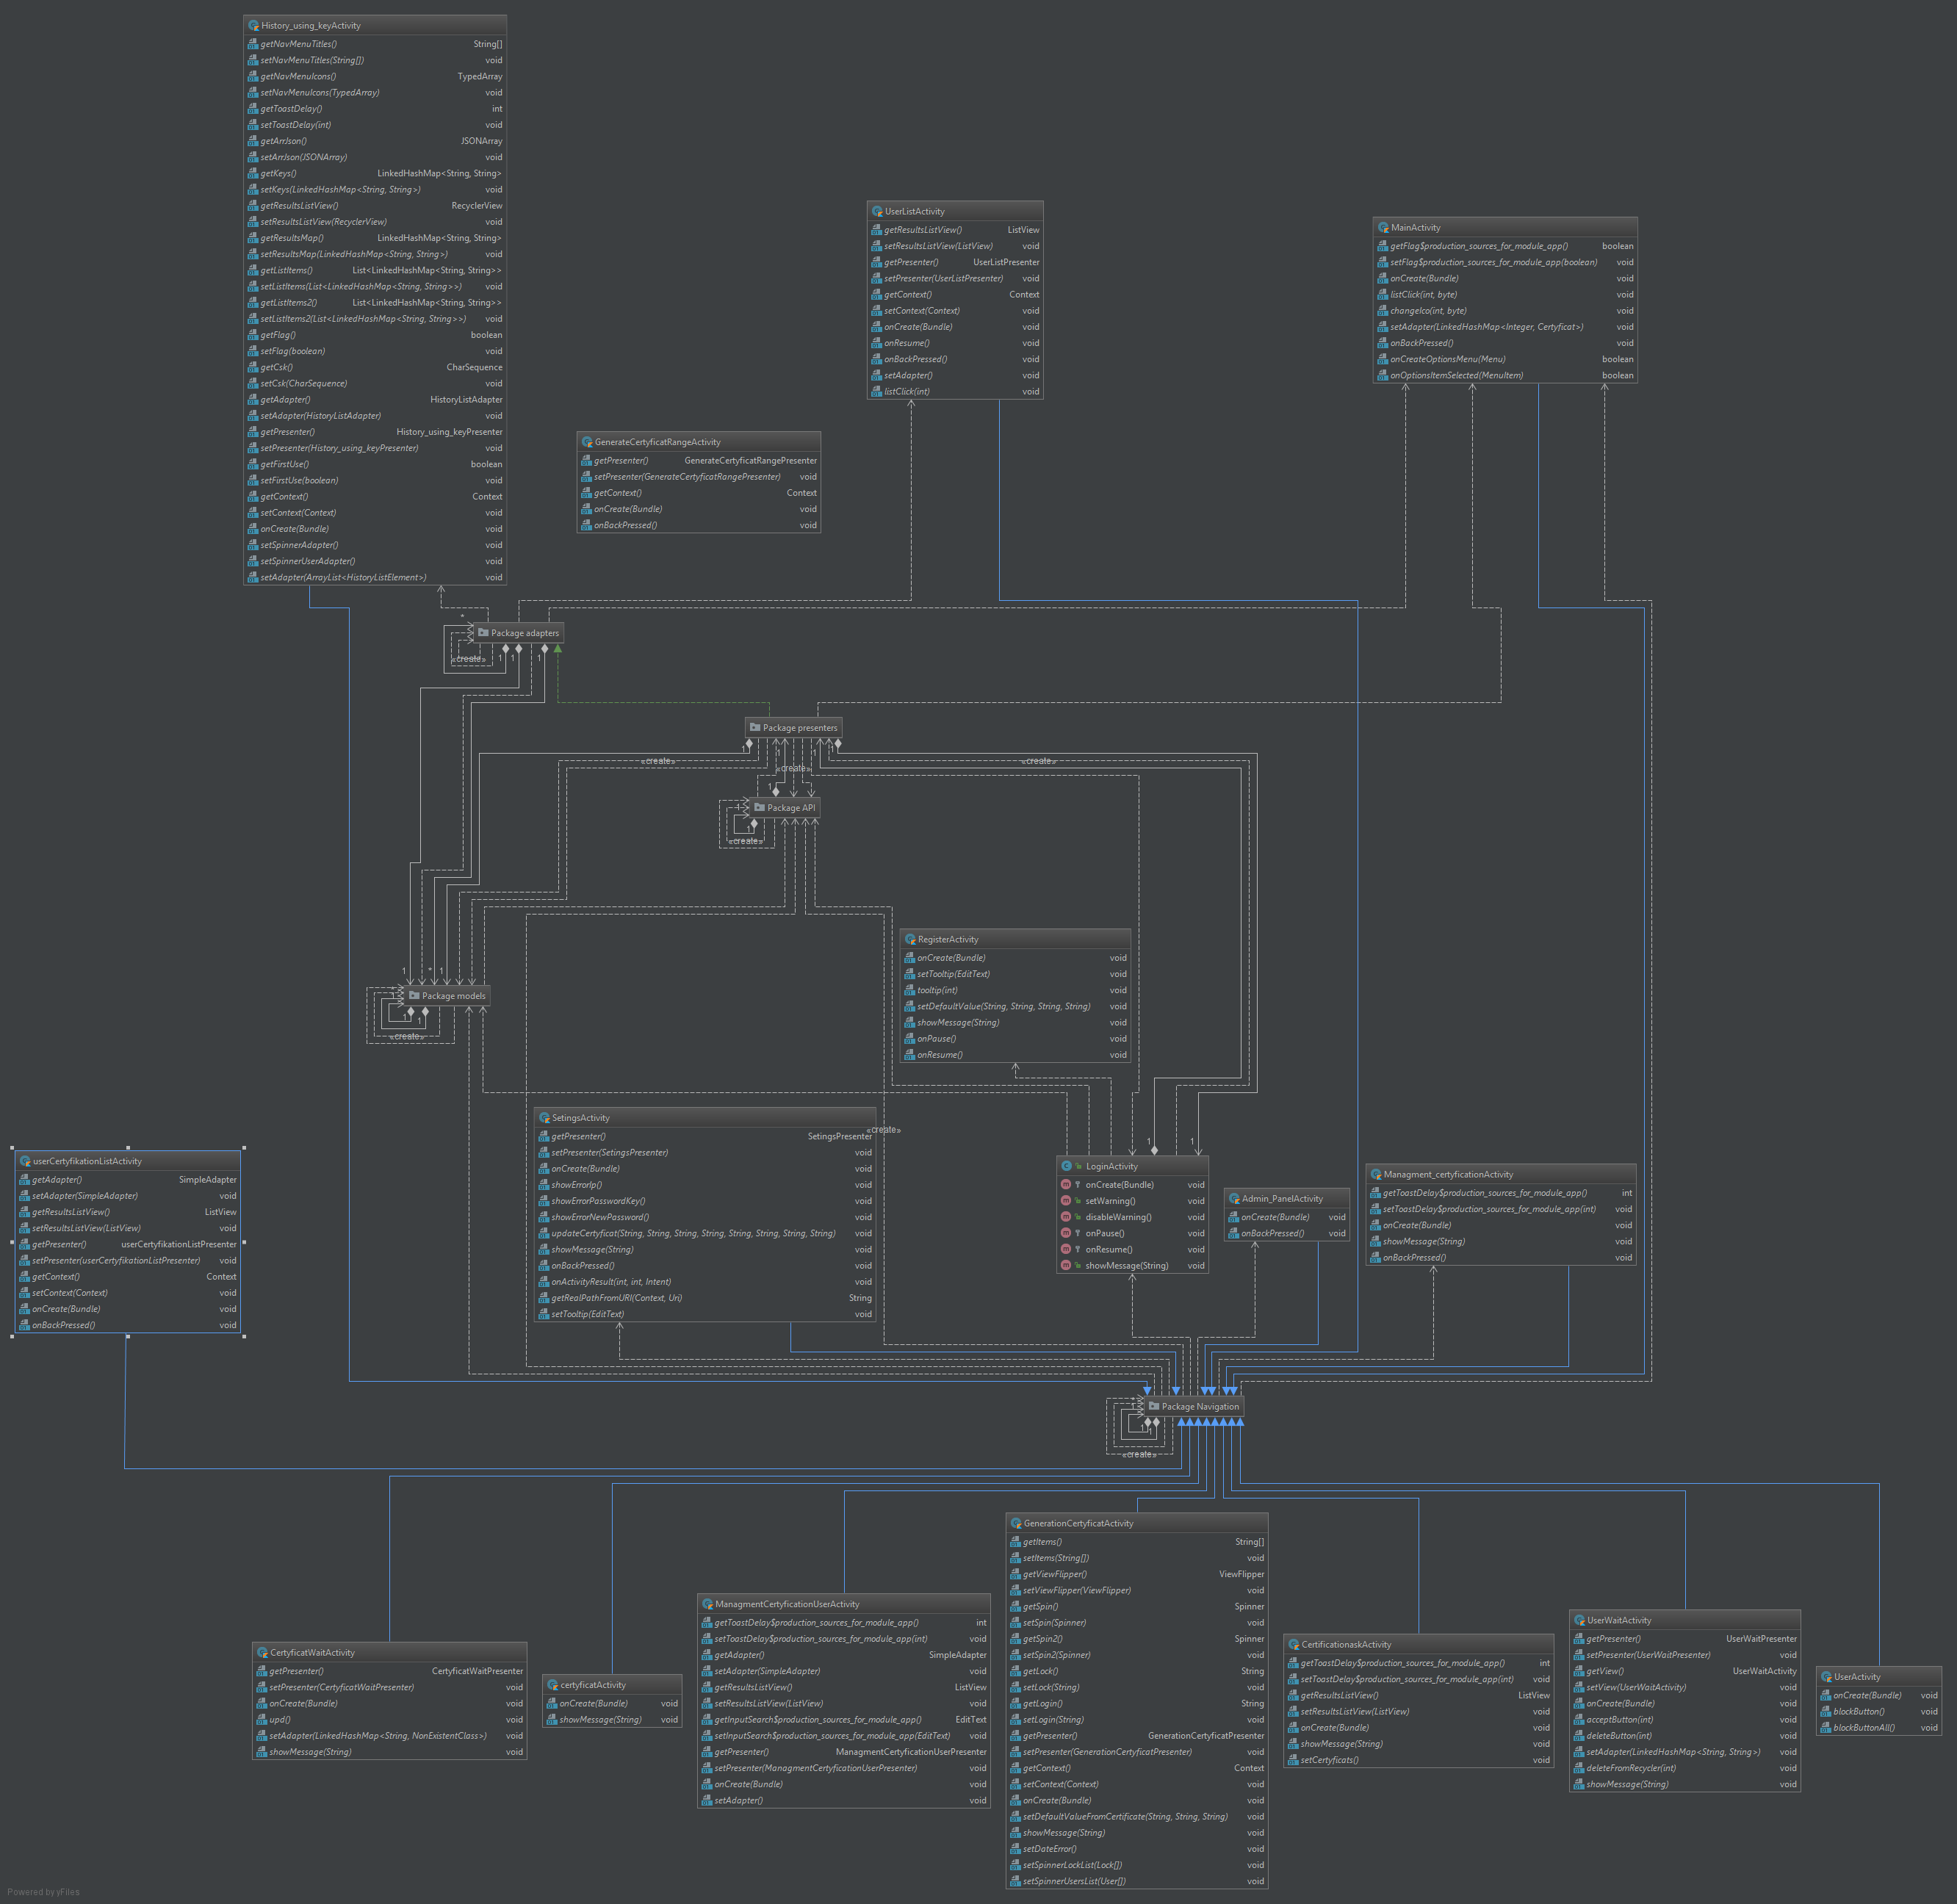
\includegraphics[width=12cm]{Obrazy/AM_DK_view}
	\caption{Diagram klas dla paczki views}
	\label{Diagram klas dla paczki views}
\end{figure}
\newpage

		\begin{figure}[ht!]
			\centering
			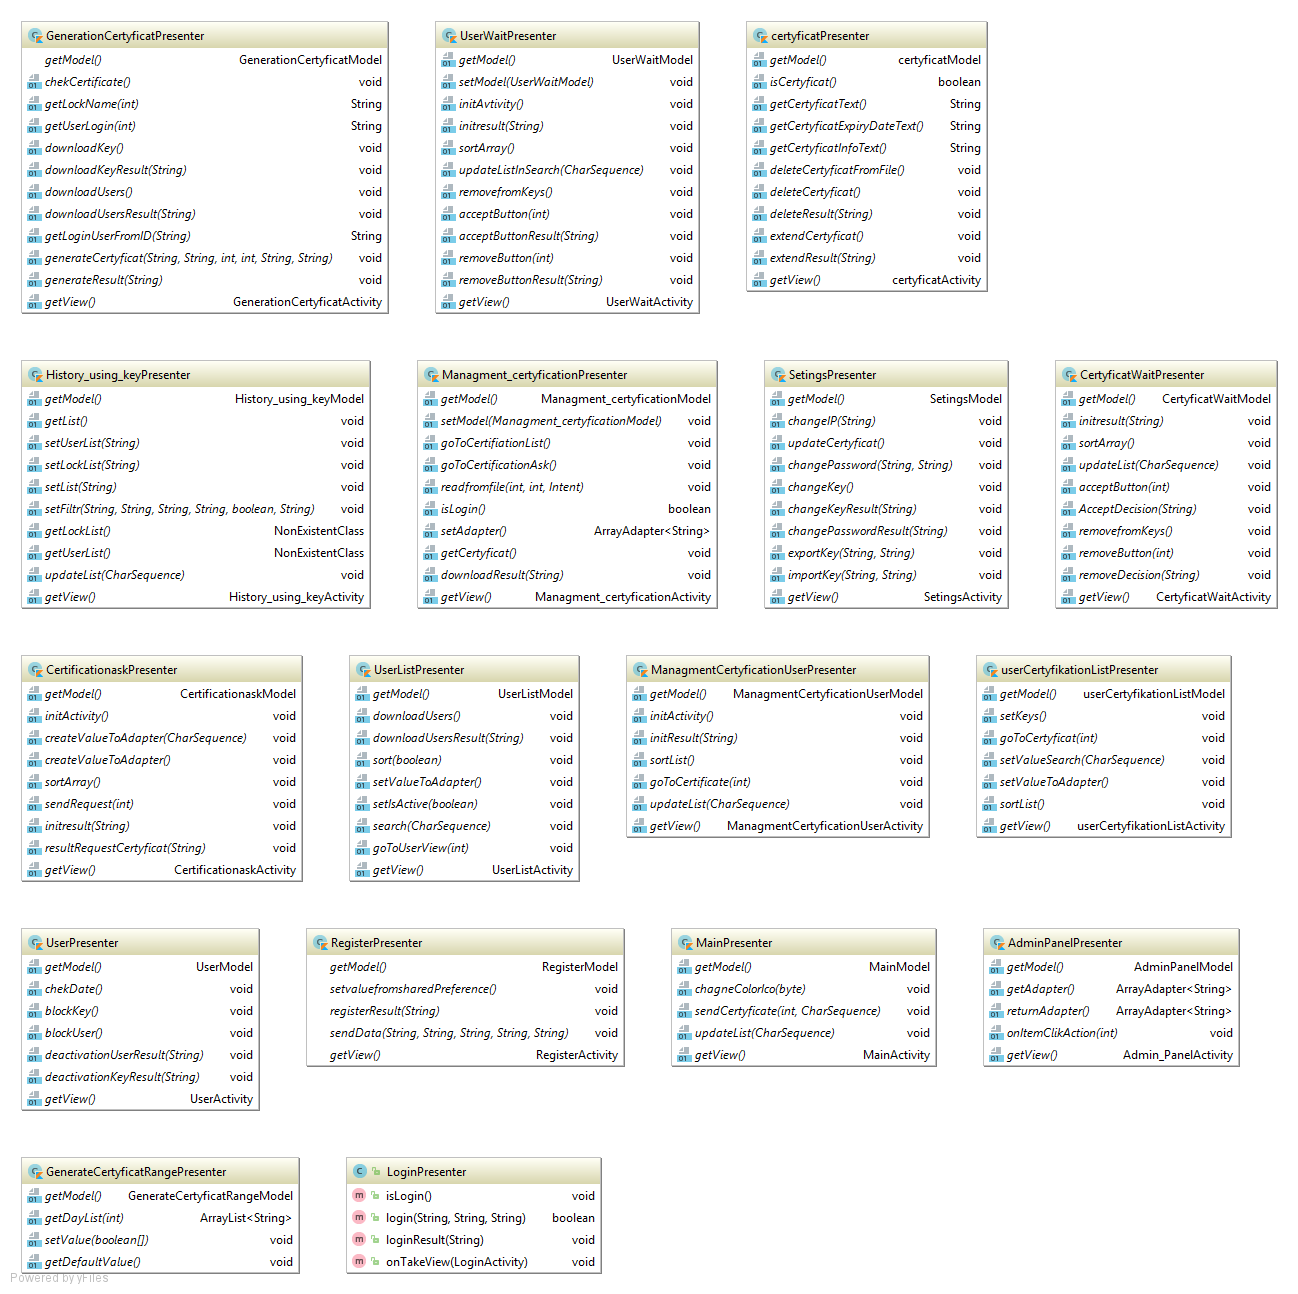
\includegraphics[width=12cm]{Obrazy/AM_DK_presenter}
			\caption{Diagram klas dla paczki presenters}
			\label{Diagram klas dla paczki presenters}
		\end{figure}
		\newpage		

		\paragraph*{Aplikacja serwera}
		
		\paragraph*{Urządzenie sterujące}
		\paragraph*{Moduł zliczania osób}

\newpage		
\subsection{Uproszczony schemat elektryczny systemu}\label{sec:Schemat elektryczny zamka}

\newpage
\subsection{Komunikacja modułów systemu z aplikacją  serwera}
	\begin{landscape}
			\subsubsection{Komunikaty HTTPRequest pomiędzy urządzeniem sterującym, a serwerem}

		
		\begin{longtable}[!ht]{|p{5cm}|p{6cm}|p{6.5cm}|p{3cm}|} 
			\caption{Tabela komunikatów HTTP dla Raspberry Pi}
			\label{tab:http_raspberry}\\
			\hline	
			Adres URL & Parametry & Odpowiedź & Opis \\	\hline
			/api/RPI/download/cerificate/ & certificate\_id --- identyfikator certyfikatu \newline RPI\_MAC --- adres MAC urządzenia \newline login\_user --- login użytkownika & "data": dict\_all\_certificate, "public\_key": public\_key \tablinia "data": "invalid" & Pobranie certyfikatu użytkownika \\ \hline
			/api/RPI/access\_decision/ & certificate\_id --- identyfikator certyfikatu \newline decision --- informacja o odmowie/akceptacji dostępu & "status": "ok" \tablinia "data": "invalid" & Informacja do serwera o statusie otwierania zamka \\ \hline
		\end{longtable}
	\end{landscape}
\newpage
\begin{landscape}
	\subsubsection{Komunikaty HTTPRequest pomiędzy aplikacją mobilną, \newline a serwerem}
	\begin{longtable}[!ht]{|m{5cm}|m{6cm}|m{6.5cm}|m{3cm}|} 
		\caption{Tabela komunikatów HTTP dla urządzenia mobilnego}
		\label{tab:http_mobilne}\\
		\hline	
		Adres URL & Parametry & Odpowiedź & Opis \\	\hline
		/api/login/ & username --- login użytkownika \newline password --- hasło użytkownika & "status": "ok", "token": token \tablinia "Status'': "ERROR PASSWORD", "token": "invalid" \tablinia "status": "not activated", "token": "invalid" & Logowanie użytkownika do aplikacji \\ \hline
		/api/register/ & login --- login użytkownika \newline password --- hasła użytkownika \newline name --- imię użytkownika \newline surname -- nazwisko użytkownika \newline publickey --- klucz publiczny użytkownika & "status": "ERROR" \tablinia "status": "REGISTER OK" & Rejestracja nowego użytkownika do aplikacji \\ \hline
		/api/logout/ & login --- login użytkownika \newline token --- klucz sesji logowania & "status": "logout" \tablinia "status": "invalid" & Wylogowanie użytkownika z aplikacji \\ \hline
		/api/download/all\_certifacate/ & login --- login użytkownika \newline token --- klucz sesji logowania & "data": dict\_all\_certificate \tablinia "status": "invalid" & Pobranie wszystkich dostępnych certyfikatów użytkownika \\ \hline
		/api/download/all\_locks/ & login --- login użytkownika \newline token --- klucz sesji logowania & "data": dict\_all\_locks \tablinia "status": "invalid" & Pobranie listy wszystkich dostępnych zamków w systemie \\ \hline
		/api/download/all\_user/ & login --- login użytkownika \newline token --- klucz sesji logowania & "data": dict\_all\_users \tablinia "status": "invalid" & Pobranie listy wszystkich użytkowników systemu \\ \hline
		/api/deactivation/ & login --- login użytkownika \newline token --- klucz sesji logowania \newline certificate\_id --- identyfikator certyfikatu do usunięcia & "status": "ok" \tablinia "status": "invalid" & Usunięcie dostępu do certyfikatu \\ \hline
		/api/request\_new\_certificate/ & login --- login użytkownika \newline token --- klucz sesji logowania \newline lock\_id --- identyfikator zamka & "status": "ok" \tablinia "status": "invalid" & Wnioskowanie o nowy certyfikat \\ \hline
		/api/change\_password/ & login --- login użytkownika \newline token --- klucz sesji logowania \newline newpasswd --- nowe hasło użytkownika & "status": "ok" \tablinia "status": "invalid" & Zmiana hasła użytkownika \\ \hline
		/api/admin/history/ & login --- login użytkownika \newline token --- klucz sesji logowania & "data": dict\_history \tablinia "status": "invalid" & Pobranie historii użycia zamków w systemie (administrator) \\ \hline
		/api/admin/download/\linebreak all\_certificate/ & login --- login użytkownika \newline token --- klucz sesji logowania & "data": dict\_all\_certificate \tablinia "status": "invalid" & Pobranie wszystkich certyfikatów z systemu (administrator)\\ \hline
		/api/admin/deactivation/ & login --- login użytkownika \newline token --- klucz sesji logowania \newline certificate\_id --- identyfikator certyfikatu do usunięcia & "status": "ok" \tablinia "status": "invalid" & Usunięcie dostępu do certyfikatu (administrator) \\ \hline
		/api/admin/register\_waiting/ & login --- login użytkownika \newline token --- klucz sesji logowania & "status": "ok" \tablinia "status": "invalid" & Pobranie listy oczekujących użytkowników na zaakceptowanie rejestracji \\ \hline
		/api/admin/register\_decision/ & login --- login użytkownika \newline token --- klucz sesji logowania \newline user\_login --- login użytkownika, którego dotyczy decyzja \newline decision --- decyzja True/False dotycząca akceptacji rejestracji & "status": "ok" \tablinia "status": "invalid" & Podjęcie decyzji przez administratora dotycząca rejestracji użytkownika o danym loginie \\ \hline
		/api/admin/certificate\_waiting/ & login --- login użytkownika \newline token --- klucz sesji logowania & "status": "ok" \tablinia "status": "invalid" & Pobranie listy oczekujących certyfikatów na zaakceptowanie \\ \hline
		/api/admin/certificate\_decision/ & login --- login użytkownika \newline token --- klucz sesji logowania \newline certificate\_id --- identyfikator certyfikatu, którego dotyczy decyzja & "status": "ok" \tablinia "status": "invalid" & Podjęcie decyzji przez administratora dotycząca przyjęcia \\ \hline
		/api/admin/\linebreak generate\_new\_certificate/ & login --- login użytkownika \newline token --- klucz sesji logowania \newline user\_id --- identyfikator użytkownika \newline lock\_id --- identyfikator zamka \newline from\_date --- data od której obowiązuje certyfikat \newline to\_date --- data do której obowiązuje certyfikat \newline monday...sunday --- 7 parametrów oznaczjacych zakresy godzin w poszczególnych dniach tygodnia \newline is\_pernament --- czy dostęp jest ciągły \newline name --- imię użytkownika certyfikatu \newline surname --- nazwisko użytkownika certyfikatu & "status": "ok" \tablinia "status": "invalid" & Generowanie nowego certyfikatu (administrator) \\ \hline
		
	\end{longtable}
\end{landscape}
	
\newpage
\subsection{Protokoły komunikacji pomiędzy urządzeniem \newline sterującym i aplikacją mobilną}

\newpage
\subsection{Interfejs graficzny systemu}\label{sec:Projekt interfejsu graficznego}
	\subsubsection{Widoki aplikacji mobilnej}
		\paragraph*{Panel logowania użytkownika}
	Widok umożliwiać będzie zalogowanie się użytkownika do systemu poprzez podanie loginu, hasła oraz adres IP serwera w odpowiednie pola, a następnie kliknięcie w przycisk “ZALOGUJ SIĘ”. Samo pole hasła będzie maskowane. Jeśli nie posiada się konta, zostanie utworzona możliwość  utworzenia konta poprzez przycisk “ZAREJESTRUJ SIĘ”. (Rysunek \ref{rys:panel_logowania_pionowo})
	
	
	\begin{figure}[ht!]
			\centering
			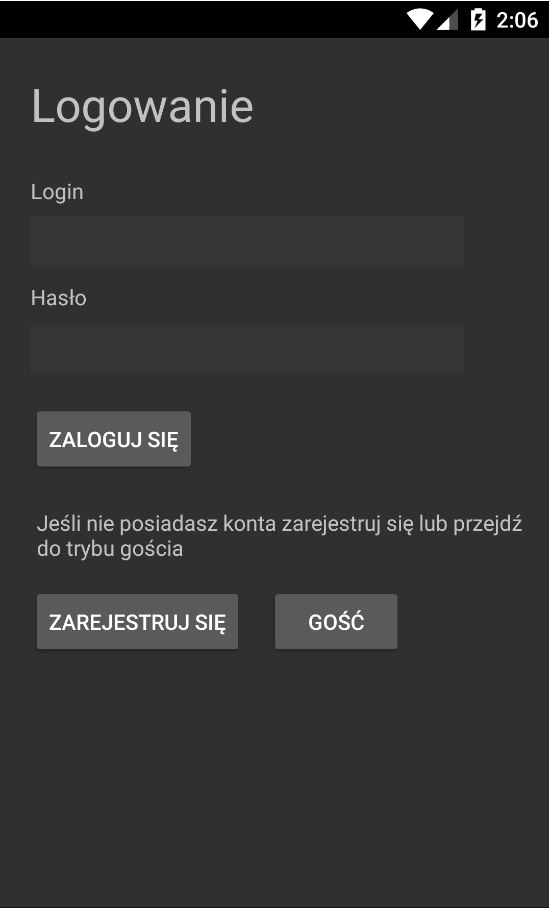
\includegraphics[width=12.5cm,height=8cm,keepaspectratio]
			{Obrazy/logowanie_uzytkownika_pionowo}
			\caption{Panel logowania użytkownika}
			\label{rys:panel_logowania_pionowo}
	\end{figure}

	
	\paragraph*{Panel rejestracji użytkownika}
	Panel rejestracji służyć będzie do utworzenie nowego użytkownika poprzez podanie loginu, hasła, imienia i nazwiska użytkownika oraz adresu IP serwera do którego chcemy się zarejestrować. Pole z hasłem będzie maskowane wraz z możliwością odkrywania hasła przy pomocy ikonki oko Po upewnieniu się, że wszystkie dane są poprawne, aby zakończyć proces rejestracji, trzeba będzie kliknać przycisk “ZAREJESTRUJ”. (Rysunek \ref{rys:panel_rejestracji_pionowo})
	
	\begin{figure}[ht!]
		\centering
		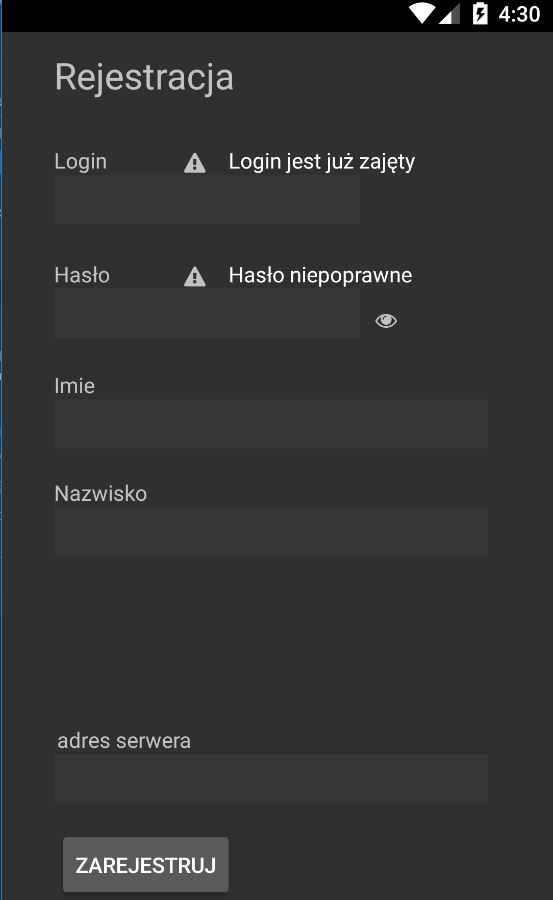
\includegraphics[width=12.5cm,height=8cm,keepaspectratio]
			{Obrazy/rejestracja_uzytkownika_pionowo}
			\caption{Panel logowania użytkownika }
			\label{rys:panel_rejestracji_pionowo}
		
	\end{figure}
	
	
	\paragraph*{Panel listy zamków}
	Widok listy dostępnych zamków przedstawia listę nazw zamków do jakich dany użytkownik ma dostęp. Ułatwieniem będzie możliwość sortowania wyników i wyszukiwanie po nazwach. Kliknięcie w nazwę zamka spowoduje otwarcie zamka. Zmiana koloru\footnote{Opisy znaczeń poszcególnych kolorów oraz symboli opisane są w rozdziale \ref{Symbolika ikon}} ikon zamków sygnalizować będzie status zamka. (Rysunek \ref{rys:panel_listy_dostepnych_zamkow_pionowo})
	
	\begin{figure}[ht!]
			\centering
		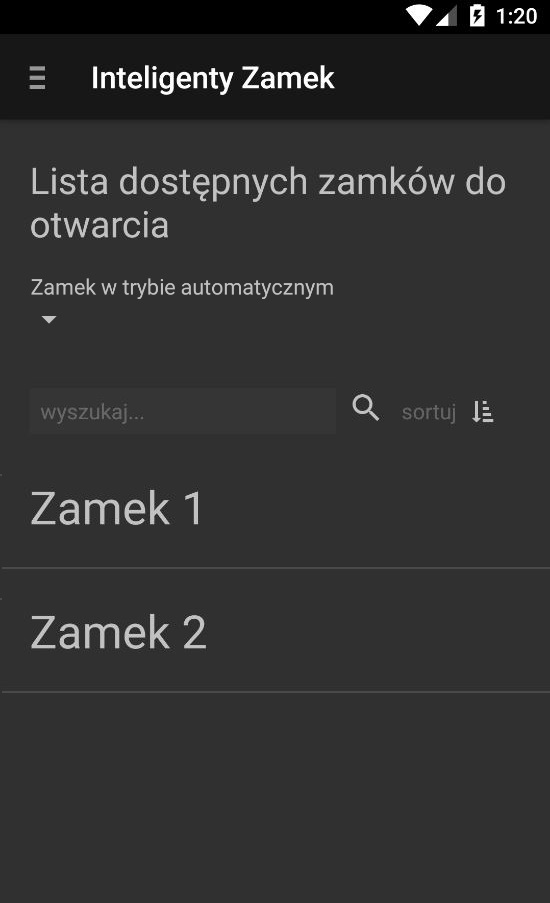
\includegraphics[width=12.5cm,height=8cm,keepaspectratio]
			{Obrazy/lista_dostepnych_zamkow_pionowo}
			\caption{Lista dostępnych zamków}
			\label{rys:panel_listy_dostepnych_zamkow_pionowo}
	
		
	\end{figure}
	
	
	\paragraph*{Panel boczny}
	Panel boczny pozwalać będzie na szybkie przełączanie pomiędzy widokami. Chowany zostanie po lewej stronie ekranu. Umożliwi przechodzenie odpowiednio do listy zamków, zarządzania certyfikatami, panelu administracyjnego oraz ustawień. Ostatnia pozycja spowoduje wylogowanie z aplikacji. Pnanel ten w zależnośći od uprawnień użytkownika możę posiadać lub nie pole z panelem administraotra (Rysunek \ref{rys:panel_boczny_pionowo} i \ref{rys:panel_boczny_pionowo2})
	
	\begin{figure}[ht!]
		\begin{minipage}{0.5\textwidth}
			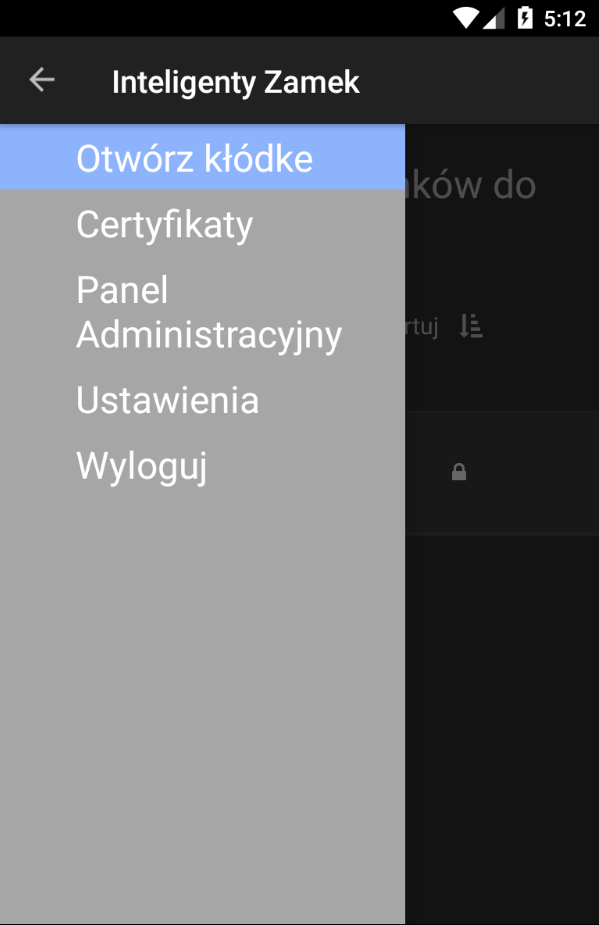
\includegraphics[width=\textwidth]
			{Obrazy/panel_boczny_pionowo}
			\caption{Panel boczny z uprawnieniami administratora}
			\label{rys:panel_boczny_pionowo}
		\end{minipage}
		\begin{minipage}{0.5\textwidth}
			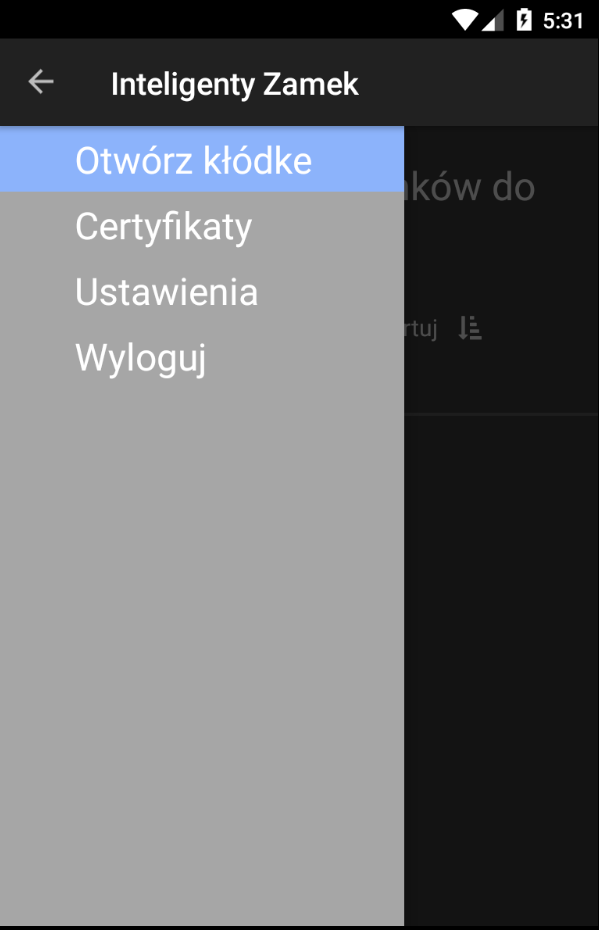
\includegraphics[width=\textwidth]{Obrazy/panel_boczny_pionowo2}
			\caption{Panel boczny bez uprawnieni administratora}
			\label{rys:panel_boczny_pionowo2}
		\end{minipage}	
	\end{figure}

	
	\paragraph*{Panel zarządzania certyfikatami}
	Panel zarządzania certyfikatami umożliwi wybór funkcji dodania certyfikatu. Kolejne pozycje to lista posiadanych certyfikatów oraz wysłanie wniosku o utworzenie nowego certyfikatu  (Rysunek \ref{rys:panel_zarządzania_certyfikatami_pionowo})
	
	\begin{figure}[ht!]
		\centering
		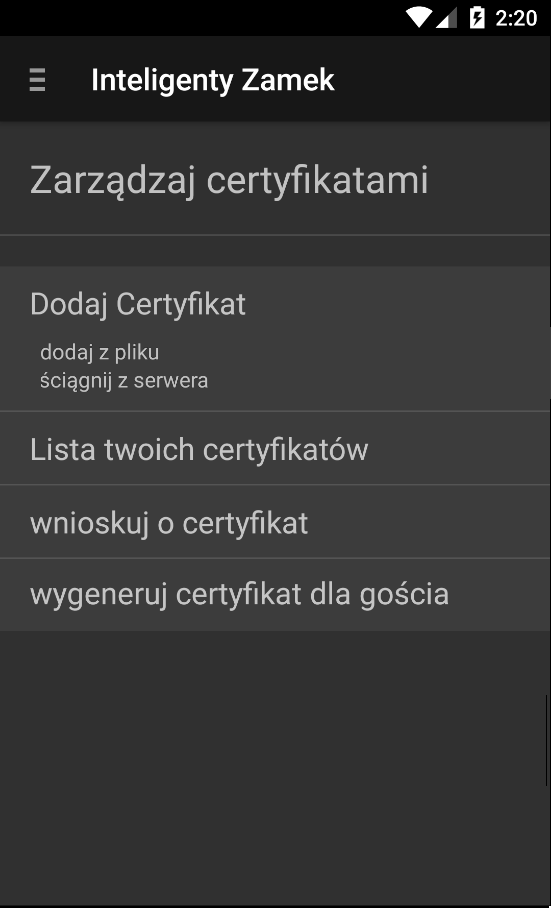
\includegraphics[width=12.5cm,height=8cm,keepaspectratio]
			{Obrazy/zarzadzaj_certyfikatami_pionowo}
			\caption{Panel zarządzania certyfikatami }
			\label{rys:panel_zarządzania_certyfikatami_pionowo}
		
	\end{figure}

	
	\paragraph*{Panel listy certyfikatów}
	Panel listy certyfikatów, będzie listą aktualnych certyfikatów należących do użytkownika. Kliknięcie w dany certyfikat przeniesie do widoku szczegółowego związanego z operacjami na tym certyfikacie. (Rysunek \ref{rys:panel_listy_certyfikatów_pionowo} )
	
	\begin{figure}[ht!]
			\centering
	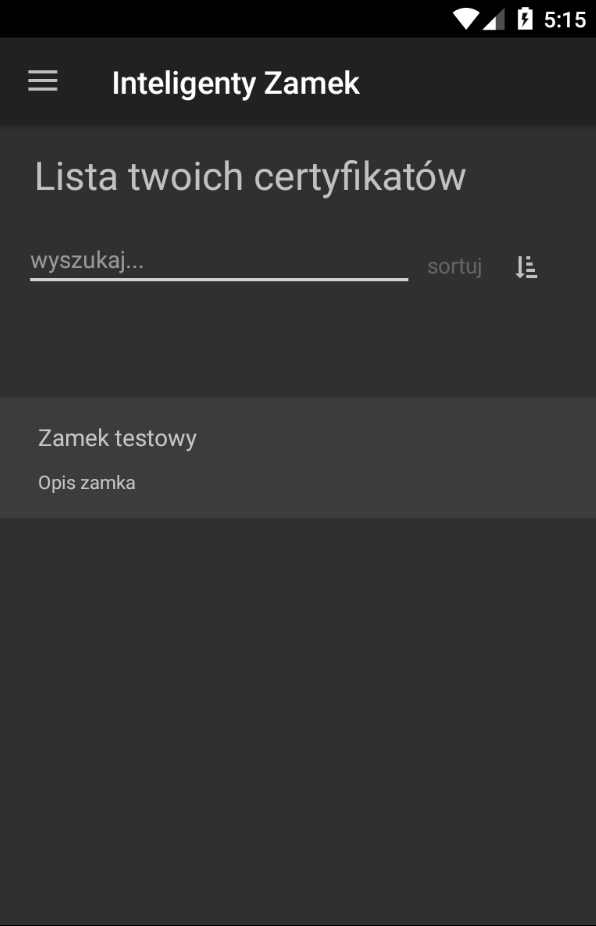
\includegraphics[width=12.5cm,height=8cm,keepaspectratio]
			{Obrazy/lista_certyfikatow_pionowo}
			\caption{Panel listy certyfikatów}
			\label{rys:panel_listy_certyfikatów_pionowo}
		
	\end{figure}

	
	\paragraph*{Panel certyfikatu}
	Panel certyfikatu zawierać będzie informacje o dacie wygaśnięcia, którego zamku dotyczy oraz w jakim czasie przyznaje dostęp. Na dole dostępne będą dwa przyciski pozwalające usunąć certyfikat lub wysłać prośbę o przedłużenie ważności. W zależnośći od tego czy uzytkownik ma uprawnienia administratora przycisk przedłuż certyfikat albo wyśle zgłoszenie do serwera (dla użytkownika bez uprawnieni administratora) albo przeniesie do panelu generowania certyfikatu (dla użytkownika o uprawnieniach administratora) (Rysunek \ref{rys:panel_certyfikatu_pionowo})
	
	\begin{figure}[ht!]
		\centering
		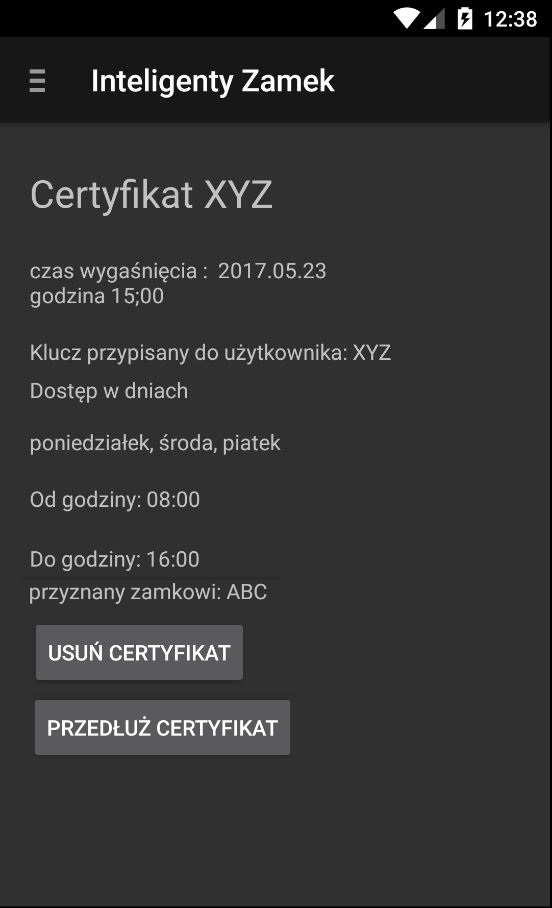
\includegraphics[width=12.5cm,height=8cm,keepaspectratio]
			{Obrazy/certyfikat_pionowo}
			\caption{Panel certyfikatu }
			\label{rys:panel_certyfikatu_pionowo}
		
	\end{figure}
	
	\paragraph*{Panel wnioskowania o certyfikat}
	Panel wnioskowania o certyfikat polegać będzie na wybraniu z listy wszystkich zamków, konkretnego do którego chcemy uzyskać dostęp i wysłaniu wniosku o przydzielenie dostępu. (Rysunek \ref{rys:panel_wnioskowania_o_certyfikat_pionowo})
	
	\begin{figure}[ht!]
		\centering
		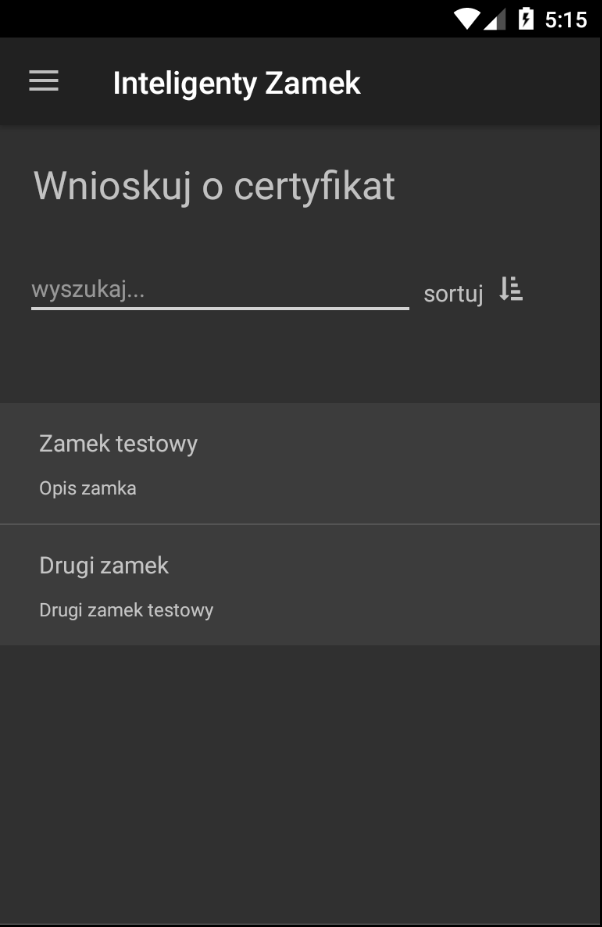
\includegraphics[width=12.5cm,height=8cm,keepaspectratio]
			{Obrazy/wnioskuj_o_certyfikat_pionowo}
			\caption{Panel wnioskowania o certyfikat }
			\label{rys:panel_wnioskowania_o_certyfikat_pionowo}
	
	\end{figure}
	
	
	\paragraph*{Panel administratora}
	W panelu administratora znajdować się będzie 6 przycisków do administrowania systemem zamków:
	\begin{itemize*}
		\item ,,Historia użycia zamków''
		\item ,,Generowanie nowego certyfikatu'',
		\item ,,Zarządzanie certyfikatami użytkowników'',
		\item ,,Lista oczekujących użytkowników do zarejestrowania'',
		\item ,,Lista oczekujących certyfikatów do zaakceptowania'',
		\item ,,Zarządzanie kontami użytkowników''.
	\end{itemize*}
	
	Po kliknięciu każdego przycisku przejdzie się do nowego odpowiadającego widoku. (Rysunek \ref{rys:panel_administracyjny_pionowo})
	
	\begin{figure}[ht!]
			\centering
	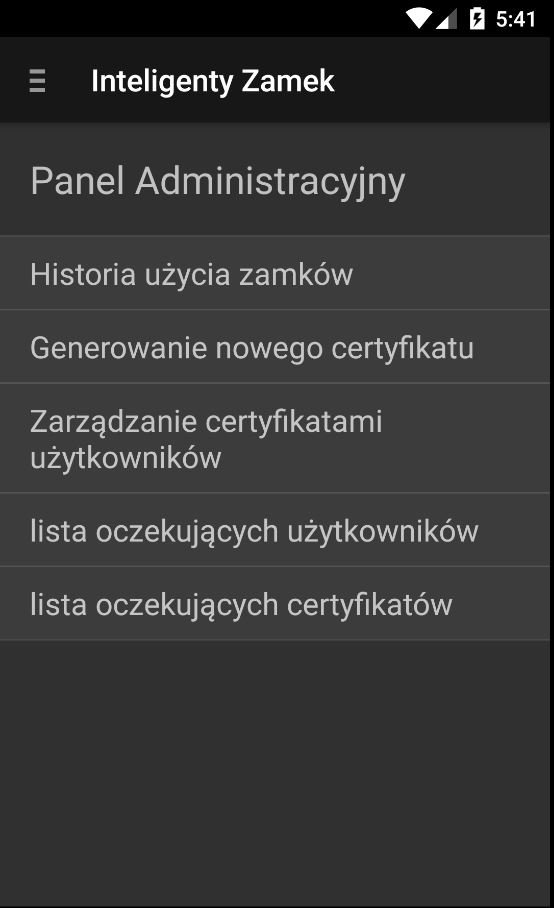
\includegraphics[width=12.5cm,height=8cm,keepaspectratio]
			{Obrazy/panel_administracyjny_pionowo}
			\caption{Panel administratora}
			\label{rys:panel_administracyjny_pionowo}
	
	\end{figure}

	
	\paragraph*{Panel historii użycia zamków}
	Panel historii użycia zamków składać się będzie z rozwijanej listy filtorwania histori składajaćej się z elementów takich jak lista dostępnych zamkóW, lista dostępnych uzytkowników, data podług której następuje filtracja oraz chekbox do zaznaczania czy tylko były nieautoryzowane próby. By uzyskać daną filtrację trzeba będzie nacisnać przycisk filtruj. Oprócz panelu do filtrowania znajdzie się również sama historia gdzie wyświetlane jestrodzaj próby otwarcia, data oraz przez kogo była ta próba podjęta. (Rysunek \ref{rys:panel_historii_uzycia_zamka_pionowo} i \ref{rys:panel_historii_uzycia_zamka_pionowo2})
	
	\begin{figure}[ht!]
		\begin{minipage}{0.5\textwidth}
			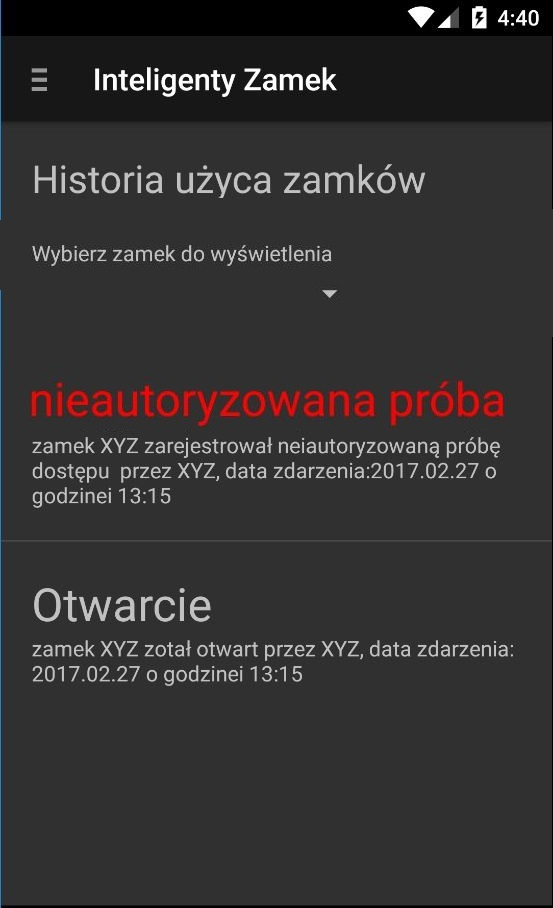
\includegraphics[width=\textwidth]{Obrazy/historia_zamkow_pionowo}
			\caption{Panel historii użycia zamków (filtr)}
			\label{rys:panel_historii_uzycia_zamka_pionowo}
		\end{minipage}
		\begin{minipage}{0.5\textwidth}
			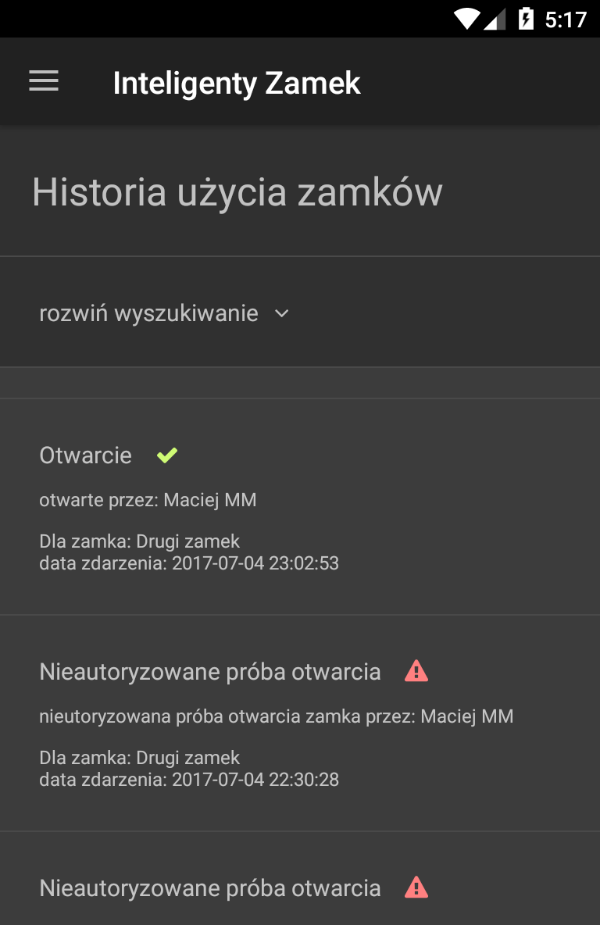
\includegraphics[width=\textwidth]{Obrazy/historia_zamkow_pionowo2}
			\caption{Panel historii użycia zamków (historia)}
			\label{rys:panel_historii_uzycia_zamka_pionowo2}	
		\end{minipage}
	\end{figure}
	\newpage
	
	\paragraph*{Panel generowania nowego certyfikatu (administrator)}
	Panel generowanie nowego certyfikatu (administrator) będzie służył do tworzenia nowych certyfikatów przez administratora. W pierwszych polach podaje się imię i nazwisko kogo dotyczy certyfikat.Następnie wybierane jest użytkownik (login) oraz zamek z rozwijanej listy. W dalszej części wybierane jest zakres dat w których certyfikat ma być ważny. Potem widać przycisk o nazwie "zakres obowiązywania certyfikatów" który przekierowywuje do widoku odpowiedzialnego za to w jakich godzinach dla danych dni tygodni certyfikat udziela dostępu. (Rysunek \ref{rys:panel_generowanie_nowego_klucza_gosc_admin_pioniowo}, \ref{rys:panel_generowanie_nowego_klucza_admin_pionowo2} i 
	\ref{rys:panel_wyboru_zakresu_certyfikatu})
	
	\begin{figure}[ht!]
		\vspace{-0.5cm}
		\begin{minipage}{0.5\textwidth}
			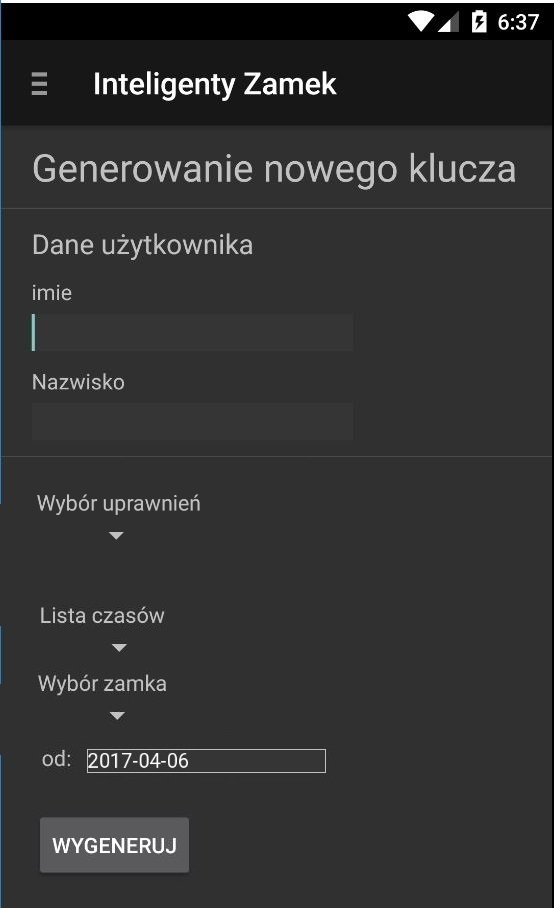
\includegraphics[width=\textwidth]{Obrazy/generowanie_nowego_klucza_gosc_admin_pioniowo}
			\caption{Panel generowania nowego klucza cz. 1 }
			\label{rys:panel_generowanie_nowego_klucza_gosc_admin_pioniowo}
		\end{minipage}
		\hspace{0.5cm}
		\begin{minipage}{0.5\textwidth}
			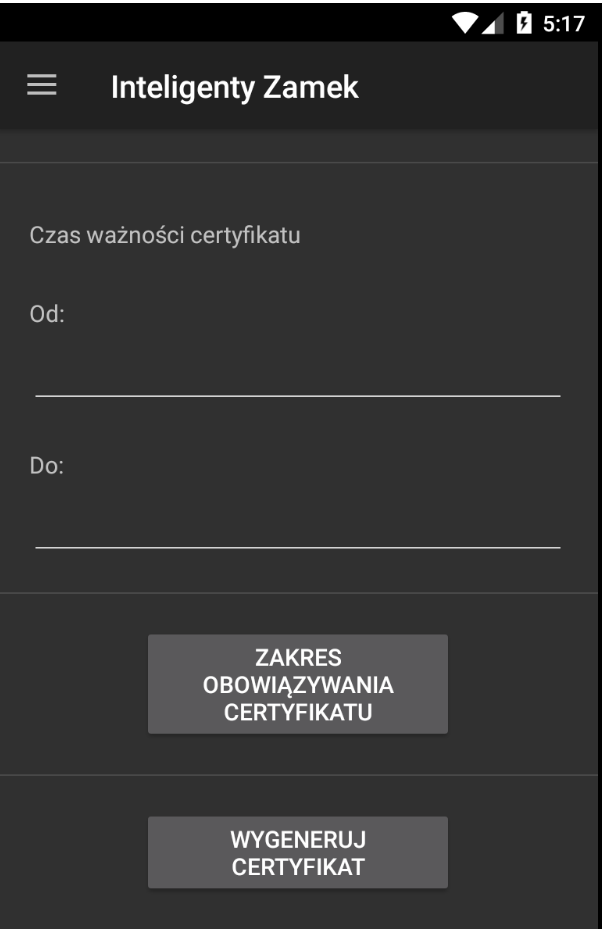
\includegraphics[width=\textwidth]{Obrazy/generowanie_nowego_klucza_admin_pionowo2}
			\caption{Panel generowania nowego klucza cz. 2}
			\label{rys:panel_generowanie_nowego_klucza_admin_pionowo2}	
		\end{minipage}
	\end{figure}
	\vspace{-0.5cm}
	\begin{figure}[ht!]
		\center
			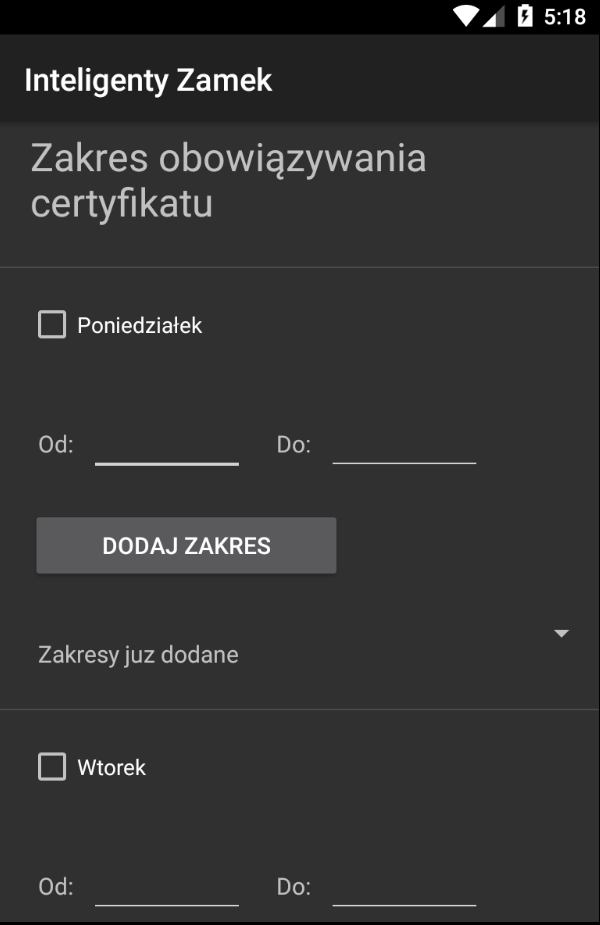
\includegraphics[width=4.5cm]{Obrazy/generowanie_nowego_klucza_uzytkownik_zalogowany_admin_pioniowo}
			\caption{Panel generowania nowego klucza dla użytkownika }
			\label{rys:panel_generowanie_nowego_klucza_uzytkownik_zalogowany_admin_pioniowo}
	\end{figure}

	
	\paragraph*{Panel zarządzania certyfikatami~(administrator)}
	Panel zarządzania certyfikatami użytkowników (administrator) będzie widokiem tylko wszystkich aktywnych certyfikatów w systemie. Administrator klikając na pozycję przejdzie do panelu certyfikatu opisanego wyżej. Tam może usunąć dostęp lub go przedłużyć. Ułatwieniem jest możliwość wyboru typu sortowania. (Rysunek \ref{rys:panel_lista_certyfikatow_administrator_pionowo})
	
	\begin{figure}[ht!]
		\centering
	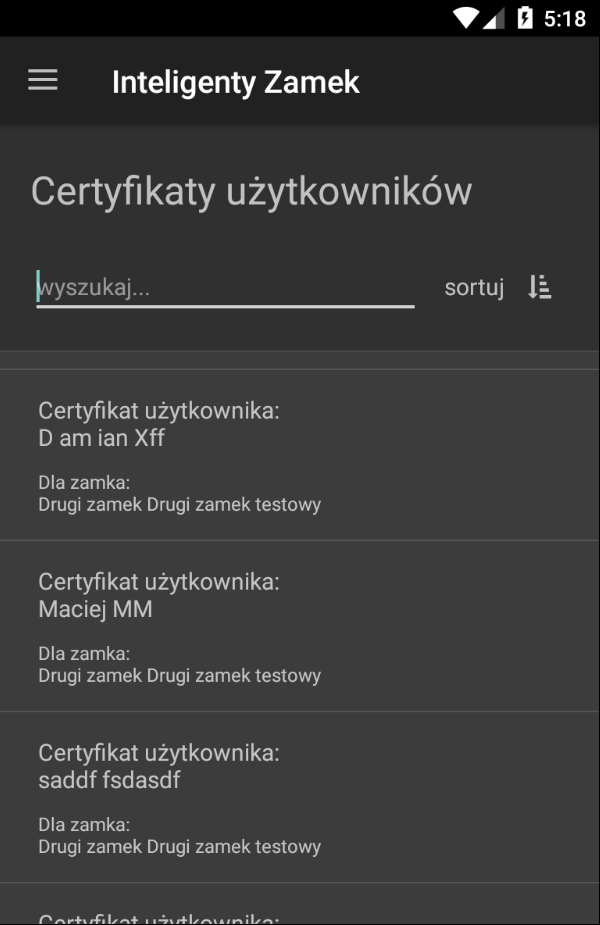
\includegraphics[width=12.5cm,height=8cm,keepaspectratio]
			{Obrazy/lista_certyfikatow_administrator_pionowo}
			\caption{Panel zarządzania certyfikatami (administrator) }
			\label{rys:panel_lista_certyfikatow_administrator_pionowo}
	
	\end{figure}

	
	\paragraph*{Panel~listy~oczekujących~użytkowników~do~rejestracji}
	Panel listy oczekujących użytkowników będzie listą wszystkich gości, którzy ubiegają się o zarejestrowanie. Po kliknięciu w odpowiednią pozycję pojawiają się dwie opcję: “AKCEPTUJ” lub “ODRZUĆ”.  (Rysunek \ref{rys:panel_lista_oczekujacych_uzytkownikow_pionowo} )
	
	\begin{figure}[ht!]
		\centering
	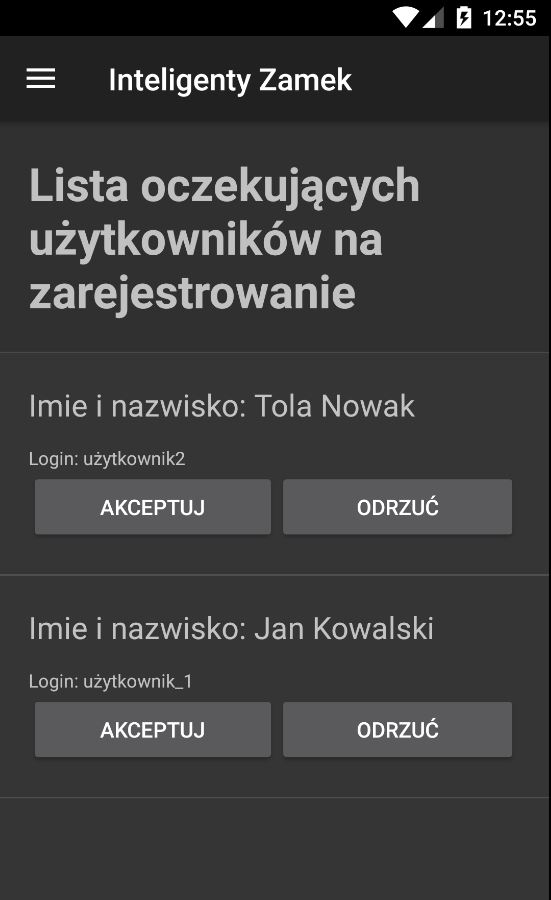
\includegraphics[width=12.5cm,height=8cm,keepaspectratio]
			{Obrazy/lista_oczekujacych_uzytkownikow_pionowo}
			\caption{Panel listy oczekujących użytkowników }
			\label{rys:panel_lista_oczekujacych_uzytkownikow_pionowo}
	
	\end{figure}

	
	\paragraph*{Panel~listy~oczekujących~certyfikatów do~wygenerowania}
	Panel listy oczekujących certyfikatów będzie listą wszystkich certyfikatów, które ubiegającyh się o akceptację administratora. Po kliknięciu w odpowiednią pozycję pojawią się dwie opcję: “AKCEPTUJ” lub “ODRZUĆ”.  (Rysunek \ref{rys:panel_lista_oczekujacych_certyfikatow_pionowo} )
	
	\begin{figure}[ht!]
			\centering
			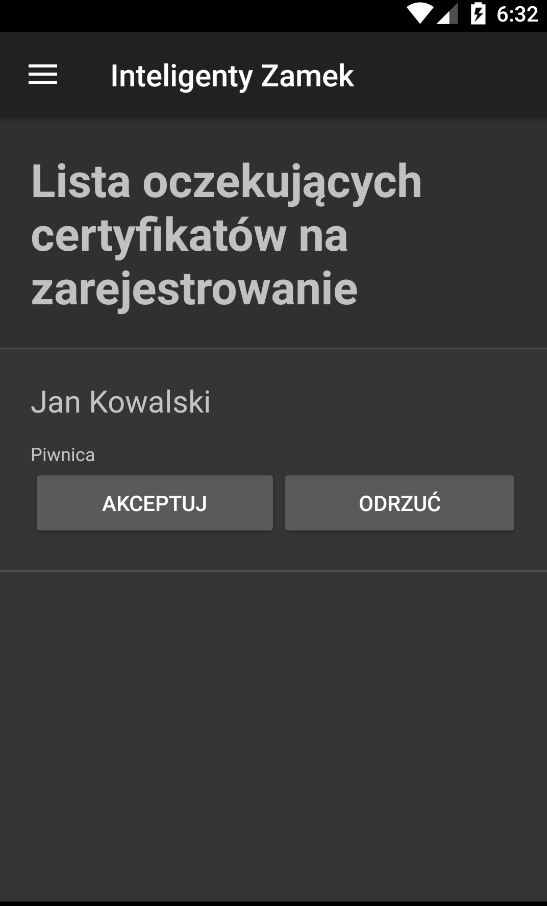
\includegraphics[width=12.5cm,height=8cm,keepaspectratio]
			{Obrazy/lista_oczekujacych_certyfikatow_pionowo}
			\caption{Panel listy oczekujących certyfikatów }
			\label{rys:panel_lista_oczekujacych_certyfikatow_pionowo}
		
	\end{figure}
	
	\paragraph*{Panel zarządzania kontami użytkowników}
	Panel ten służyć będzie do zarządzania kontami użytkowników. Wyświetli on listę użytkowników systemu wraz z z oznaczeniami czy jest on aktyny bądż zablokowany oraz czy ma ważny klucz szyfrujący (Rysunek \ref{rys:panel_Zarządzania_Kontami})
	
	\begin{figure}[ht!]
			\centering
			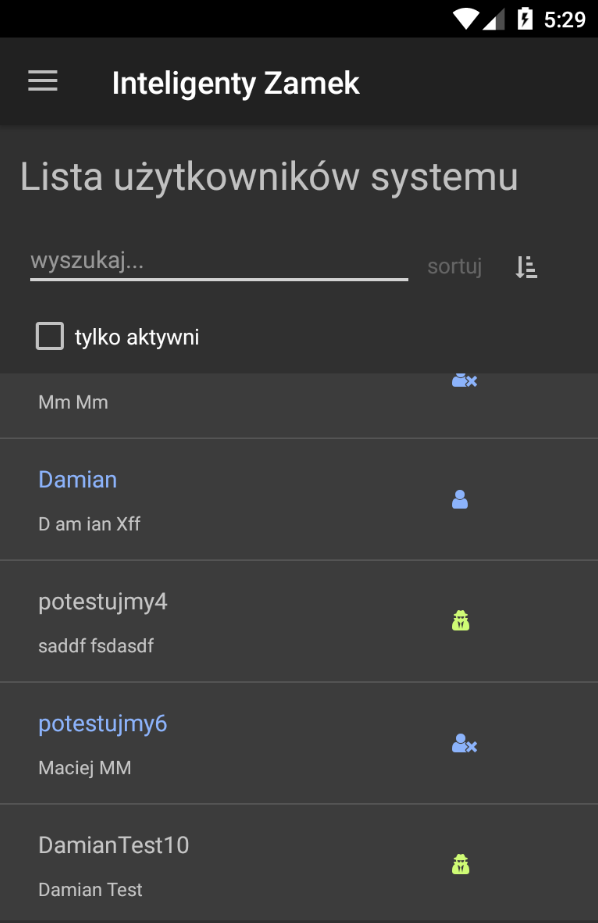
\includegraphics[width=12.5cm,height=8cm,keepaspectratio]
			{Obrazy/zarzadzanie_kontami}
			\caption{Panel zarządzania kontami użytkowników}
			\label{rys:rys:panel_Zarządzania_Kontami}
		
	\end{figure}
	
	\paragraph*{Panel ustawień konta}
	W panelu ustawień użytkownik będzie mógł zmienić hasło do swojego konta. Wymaga podania starego hasła, a następnie nowego. Ponadto w panelu tym będzie podgląd certyfikatu szyfrujaćego wraz z możliwością wygenerowania nowego oraz zmiane adresu ip serwera  (Rysunek \ref{rys:panel_ustawienia_pionowo} i \ref{rys:panel_ustawienia_pionowo2} i \ref{rys:panel_ustawienia_pionowo3})
	
	\begin{figure}[ht!]
			\centering
			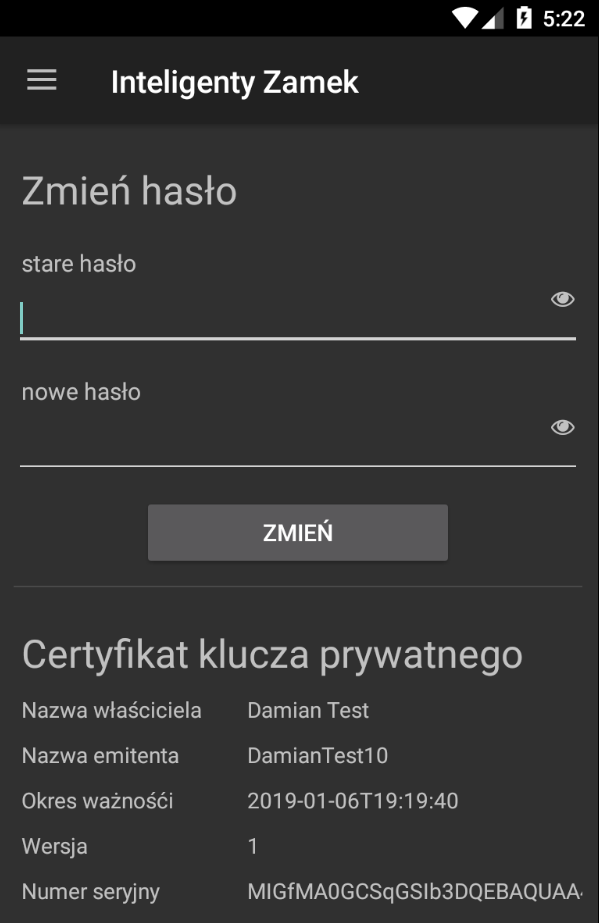
\includegraphics[width=12.5cm,height=8cm,keepaspectratio]
			{Obrazy/ustawienia_1}
			\caption{Panel ustawień konta (zmiana hasła)}
			\label{rys:panel_ustawienia_pionowo}
	\end{figure}
	\begin{figure}[ht!]
			\centering
		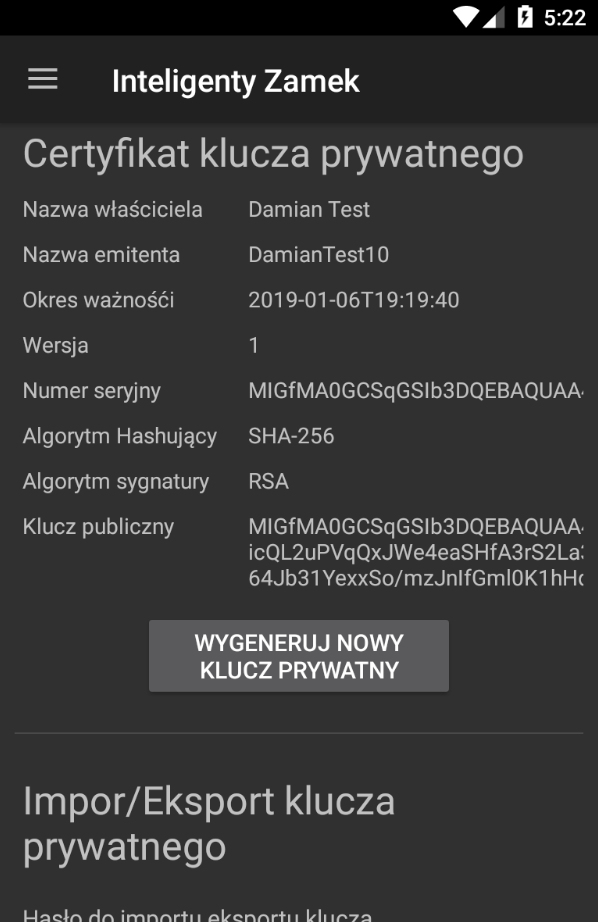
\includegraphics[width=12.5cm,height=8cm,keepaspectratio]
	{Obrazy/ustawienia_2}
	\caption{Panel ustawień konta (certyfikat szyfrująćy)}
	\label{rys:panel_ustawienia_pionowo2}
\end{figure}
	\begin{figure}[ht!]
			\centering
		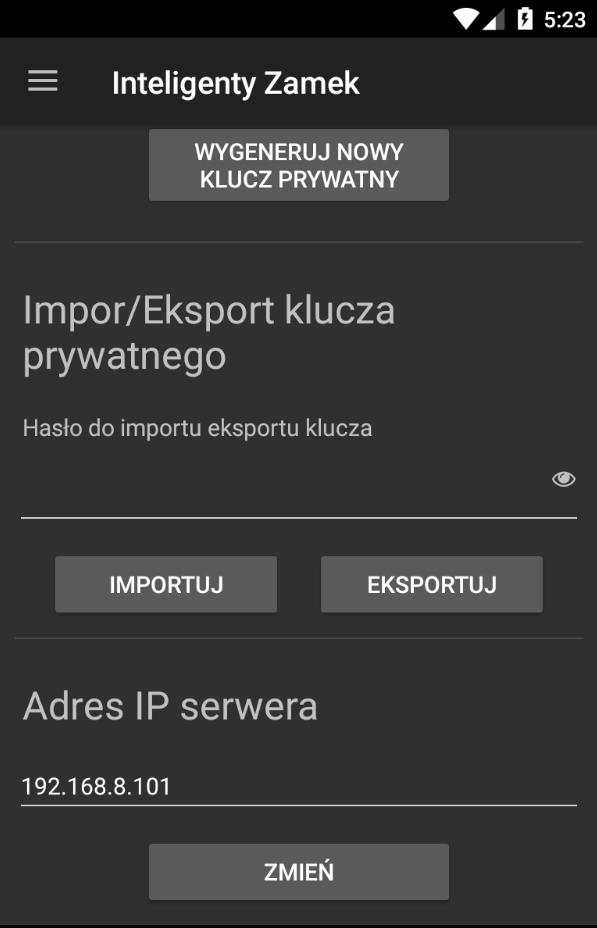
\includegraphics[width=12.5cm,height=8cm,keepaspectratio]
	{Obrazy/ustawienia_3}
	\caption{Panel ustawień konta (adres ip)}
	\label{rys:panel_ustawienia_pionowo3}
\end{figure}
	\newpage
	
	
	
	
	\subsubsection{Widoki strony internetowej systemu}
	Strona internetowa posiadć będzie dwa widoki. Jeden to widok logowania  (Rysunek \ref{rys:strona_1} w któym administrator musi wpisać login oraz hasło. W drguim widoku mamy listę histori otwarcia zamków  (Rysunek \ref{rys:strona_2}) wraz z zaznaczeniem kolorystycznym która pokazuje czy była to próba autoryzowana.
	

\begin{figure}[ht!]
		\centering
	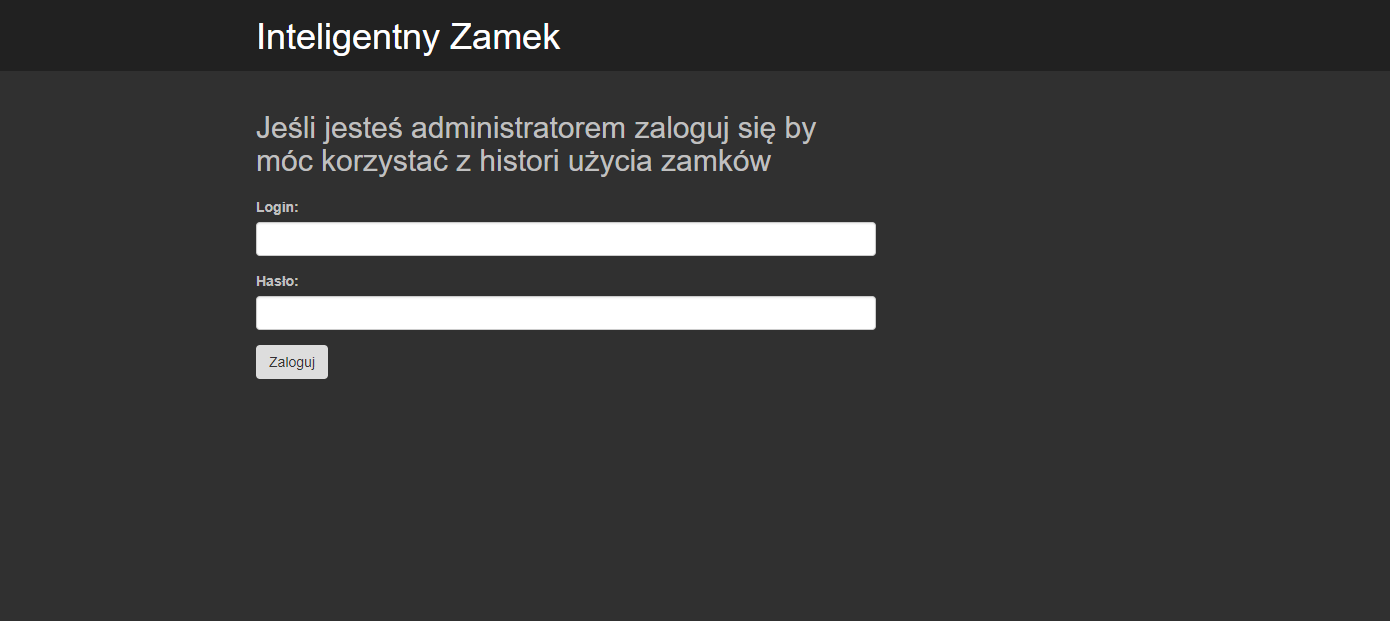
\includegraphics[width=12.5cm,height=10cm,keepaspectratio]
{Obrazy/strona_logowanie}
\caption{Strona logowania}
\label{rys:strona_1}
\end{figure}


\begin{figure}[ht!]
		\centering
	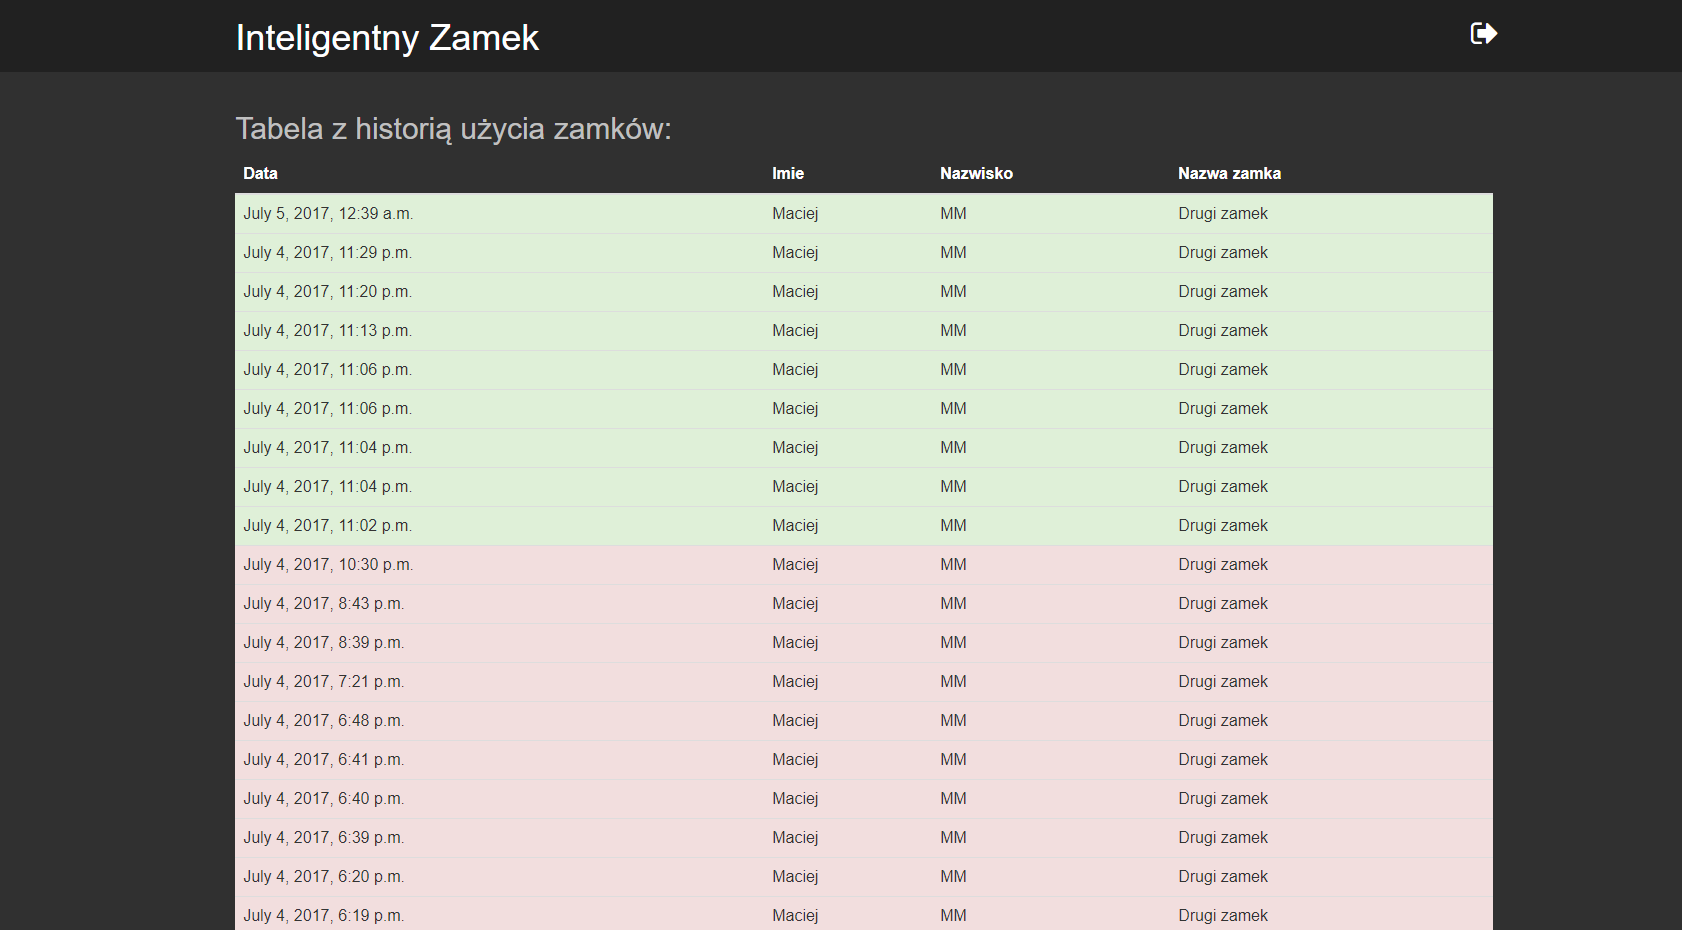
\includegraphics[width=12.5cm,height=10cm,keepaspectratio]
{Obrazy/strona_historia}
\caption{Strona z wyświetloną historią użycia zamkóW)}
\label{rys:strona_2}
\end{figure}
	
	\subsubsection{Komunikacja człowiek-interfejs}
	
		\paragraph*{Komunikaty tekstowe}
			 W aplikacji mobilnej komunikaty są wyświetlane przy pomocy toast. Komunikaty te  trwają na ekranie 4 sekundy. Informują one użytkownika o zaistniałych sytuacjach takich jak
			 \begin{itemize}
			 	\item błąd połaczenia z bazą danych
			 	\item informacja o zablokowanym koncie 
			 	\item informacja o czynnośćiach dodania bądż usunięcia odpowiednio użytkownika bądż certyfikatu
			 	\item o pobraniu listy certyfikatów
			 \end{itemize}
		 Dodatkowo są wyświetlane na ekranie komunikaty tekstowe przy pomocy  textview odnośnie walidacji danych oraz podpowiedzi podczas wpisywania haseł przy pomocy tooltip-ów ktore informuje użytkownika o paramterach jakie hasło powinno mieć
		\paragraph*{Symbolika ikon}
		Aplikacja mobilna oraz strona internetowa korzysta z symboli zawartych w fontwesome. oto poszcególne znaczenia dla danych ikon:
	   
	   
	   	\begin{longtable}[!ht]{|m{2cm}|m{10cm}|} 
	   	\caption{Tabela ikon używanych w systemie}
	   	\label{tab:ikony}\\
	   	\hline	
	   	Ikona & Opis   \\	\hline
	   	
	  
\includegraphics[width=1.5cm,height=0.7cm,keepaspectratio]{Obrazy/full_user} 	&  	ikona oznaczająca użytkownika  aktywnego z atkualnym kluczem szyfrującym 	 
	   	\\	\hline
	   	
\includegraphics[width=1.5cm,height=0.7cm,keepaspectratio]{Obrazy/user} & 	ikona oznaczająca użytkownika  aktywnego z nieatkualnym kluczem szyfrującym \\	\hline
	   		
\includegraphics[width=1.5cm,height=0.7cm,keepaspectratio]{Obrazy/block_user}&ikona oznaczająca użytkownika zablokowanego \\	\hline
	   	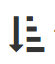
\includegraphics[width=1.5cm,height=0.7cm,keepaspectratio]{Obrazy/sort_desc}&ikonka oznaczająca sortowanie od a do z		
	   	\\	\hline				
	   	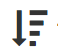
\includegraphics[width=1.5cm,height=0.7cm,keepaspectratio]{Obrazy/sort_asc}&Ikonka oznaczająca sortowanie od z do a
	   	\\	\hline
	   	
\includegraphics[width=1.5cm,height=0.7cm,keepaspectratio]{Obrazy/oko_1}	&	ikonka służąca do  pokazania na ekranie hasło które było wcześniej zamaskowane
	   	\\	\hline
	    
\includegraphics[width=1.5cm,height=0.7cm,keepaspectratio]{Obrazy/oko_2}&Ikonka służąca do maskowania hasła
	   	\\	\hline
	   	
\includegraphics[width=1.5cm,height=0.7cm,keepaspectratio]{Obrazy/menu}&Ikonka służąca do rozwijania menu
	   	\\	\hline
	   	
\includegraphics[width=1.5cm,height=0.7cm,keepaspectratio]{Obrazy/menu}&Ikonka służąca do chowania menu
	   	\\	\hline
	   	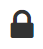
\includegraphics[width=1.5cm,height=0.7cm,keepaspectratio]{Obrazy/lock}&Ikonka oznaczająca zamknięty zamek
		\\	\hline		
	   	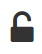
\includegraphics[width=1.5cm,height=0.7cm,keepaspectratio]{Obrazy/lock_2}&Ikonka oznaczająca otwarty zamek
	   	\\	\hline					
	   	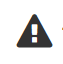
\includegraphics[width=1.5cm,height=0.7cm,keepaspectratio]{Obrazy/error}&Ikonka oznaczająca niepoprawnść np. niepoprawne hasło
	   \\	\hline
	   
\includegraphics[width=1.5cm,height=0.7cm,keepaspectratio]{Obrazy/ok}&oznaczająća poprawność np. poprawny dostęp do pomieszczenia	
	   	\\	\hline				
	   					
	   \end{longtable}
	   

	
		\paragraph*{Znaczenie kolorystyki}
		W systemie występują 4 kolory informujące użytkownika o zaistniałych sytuacjach
		\begin{itemize}
			\item czerwony który w zależnośći od kontekstu sugeruje albo niepoprawne wpisane dane, nie uzyskanie dostępu do pomieszcenia albo nieautoryzowaną próbę dostępu do pomieczenia,
			\item zielony który w zależnośći od kontekstu sugeruje poprwane uzyskanie dostępu do pomiezsceń, autoryzowaną próbę dostępu do pomieszczenia lub użytkownika który jest aktywny oraz posiada aktualny klucz szyfrujący,
			\item żółty sugeruje w naszym systemie oczekiwanie na zdarzenie,
			\item kolor fioletowy określa użytkownika który nie ma dostępu do funkcji systemu (w zależnosci od ikony ma nieaktualny klucz szyfrujący lub ma konto zablokowane)
		\end{itemize}
		
	\subsubsection{Kolorystyka systemu}
	Kolorystyka systemu została oparta o styl material design któy jest dostępny dla systemu android od wersji 5.0. Strona jak i palikacja mobilna są zbliżone kolorystycznie. Różnice w kolorach są spowodowane tylko narzuconą kolorystyką z biblioteki Bootsrap.
	
\newpage
\subsection{Bezpieczeństwo systemu}\label{sec:Projekt bezpieczeństwo}
	\subsubsection{Projekt infrastruktury klucza publicznego (PKI)}\label{sec:Projekt PKI}
		\paragraph*{Idea PKI}
		Ideą infrastruktury klucza publicznego jest zarządzanie cyfrowymi certyfikatami i kluczami szyfrującymi dla osób, oprogramowania, urządzeń i systemów. Przy jednoczesnym zahowaniu integralnośći, poufnośći oraz dostępnośći.
		\paragraph*{Urzędy certyfikujące}
		W prrzypadku \NazwaSys urzędem certyfikującym 
		\paragraph*{Klient systemu}
		W prrzypadku \NazwaSys klientem systemu będzie Aplikacja mobilna. Będzie ona odpowiedzialna za uwierzytelnianie uzytkownika w systemie oraz generowanie klucza szyfrujacego, który zostanie po tym fakcie wysyłany do urzędu certyfikującego. Sam klucz szyfrujący będzie tworzony w momecnie rejestracji uzytkownika oraz na żadanie użytkownika.
		 %nie jestem pewien czy tutaj czy w rozdziale Bezpieczeńśtwo to co poniżęj jest%
		 
		Aplikacja będzie przechowywać newralgiczne dane systemu takie jak hasło uzytkownika, jego token oraz klucz szyfrujacy. Kluczową kwestią jest odpowiednie przechowywanie tych danych w telefonie tak by nie mógł nikt niepowołany ich uzyskać. Hasło przechowywane będzie w pamieći telefonu w postaci zaszyfrowanego pliku. Plik ten będzie szyfrowany kluczem wszytym w oprogramowanie aplikacji za pomocą metody AES. Token użytkownika oraz klucz szyfrujacy będzie przechowywany jako plik w smartphonie. Plik ten będzie szyfrowany hasłem użytkownika. Dzięki temu nawet jeżeli niepowołana osoba uzyska dostęp do danych plikóW nie będzie w stanie ich odszyfrować.
		
		Drugim newraligcznym punktem aplikcaji mobilnej będzie transmisja danych dlatego w komunikacji pomiędzy serwerem a urządzeniem mobilnym wykorzystany będzie protokół HTTPs. Co uniemożliwi podsłuch danych.
	\subsubsection{Poufność}
	Poufność zostanie zapewniona przy pomocy odpowiedniego przechowywania danych a kliencie systemu, bezpiecznej wymianie danych dzięki transmisji z wykorzystaniem SSL pomiędzy modułąmi systemu oraz funkcją uwierzytelniajaćym w aplikacji mobilnej oraz na serwerze dzięi którym, dane poufne nie trafia. w niepowołane ręce. 
	\subsubsection{Dostępność}
	Dzięki popularnośći aplikacji mobilnych nasz system będzie w dużym stopniu dostępny dla użytkowników systemu. Jedynymi zagrożeniami będzie awaria sieci komputerowej w któej znajdować będzie się system oraz awaria sieci elektrycznej. Pierwsze jak i drugie zagrożenie będziemy redukować w postaci ożliwośći uzyskania dostępu do pomieszceni w tradycyjny sposób przy pomocy kluczy. Ponadto drugie zagrożenie będzie też redukowane przy pomcy urządzeni awaryjnego zasilania, co umożliwi funkcjonownaie systemu po zaniku napięcia w sieci elektrycznej przez określony czas. 
	\subsubsection{Integralność}